\documentclass[letterpaper,11pt]{article}
\usepackage[margin=1.5in]{geometry}
\usepackage[english]{babel}
%\usepackage{blindtext}
\usepackage{multicol}
%\usepackage{fullpage}
%\usepackage{mathtools}
%\usepackage{xcolor}
%\usepackage[left=3cm,top=3cm,right=3cm,nohead,nofoot]{geometry}
%\usepackage{amsmath, amssymb, graphicx, color, array, appendix}
%\usepackage[T1]{fontenc}
\usepackage[utf8]{inputenc}
%\usepackage{sistyle}
\usepackage{caption}
%\usepackage{soul}
\usepackage{hyperref}
%\usepackage{listings}
%\usepackage{verbatim}
%\usepackage{calc}
%\usepackage{graphics}
%\usepackage{wrapfig}
\usepackage{amsthm}
\usepackage{amsmath}
\usepackage{graphicx}
%\usepackage{cite}
%\usepackage{biblatex}
%\usepackage{bibtex}
%\lstset{language=C}



\linespread{1.3}
%\setlength{\hoffset}{0.5in}
\newcommand{\ud}{\,\mathrm{d}}

%Title section
\title{A Two Field Model of Inflation with a Transverse Instability}
\author{Thomas Morrison\\ Supervisors: J. Richard Bond and Jonathan Braden}
\begin{document}
\maketitle
%\tableofcontents
\begin{abstract}
%A model of inflation with both a longitudinal and a transverse field is explored in which the longitudinal field drives inflation while the transverse field experiences a temporary instability.
A two field model of inflation is explored in which, while inflation is driven by the longitudinal field, the transverse field experiences a temporary instability.The evolution of the system during inflation is calculated by making use of a lattice simulation. The change in $\zeta$ as sourced by the gradient terms in the transverse field generated during its instability is calculated.
\end{abstract}
\section{Introduction}
Inflation, referring to a period of accelerating expansion in the early universe, has been found to have a great deal of power in explaining some peculiarities in the universe we observe today. 
Inflation was first proposed as a mechanism to explain away the so called horizon and flatness problems \cite{guth81}. The horizon problem is that regions of the universe which would seemingly, without a period of inflation, be causally disconnected are observed to have a high degree of homogeneity, this homogeneity is evidenced by the near uniformity of the cosmic microwave background. Inflation alleviates the horizon problem by allowing for regions of the universe which at early times were causally connected to gain a degree of homogeneity through causal mechanisms before the accelerating expansion of the universe ends the causal contact between these regions. The flatness problem is that, in a situation where the expansion of the universe is not accelerating, a solution to a homogeneous and isotropic universe is predicted to be driven away from flat when the energy density is different from a critical value. To avoid an appeal to fine tuning parameters in order to create a flat universe, some mechanism capable of having made the universe close enough to being flat at some time in the past that it has not deviated significantly from flat at the present time is required. Such a mechanism is provided by inflation when we consider that accelerated expansion is equivalent to changing the characteristic scale over which curvature of the universe is measured, inflation then sets conditions in the past when the universe is close to flat by changing the characteristic scale over which curvature is measured.

Since its original proposal, inflation has also provided an explanation for the origin of structure in the universe in terms of curvature perturbations. Due to the expansion of the universe different regions of space become causally disconnected during inflation and curvature perturbations remain between these causally disconnected regions. After the end of inflation when regions, once causally disconnected, come back into causal connection the curvature perturbations act to seed the formation of structure.\cite{liddle}

Given the fruitfulness of inflation in explaining the universe as we see it today, investigations into inflation are of particular interest. In the present work we examine the effects of an instability during inflation acting perpendicular to the inflaton field. The remainder of this report is divided as follows: in section \ref{theory} an overview of the relevant theory is presented, in section \ref{computation} general features of the computational techniques are discussed, section \ref{two field} presents the results of lattice simulation of a two field inflation model including an instability, and concluding remarks are given in section \ref{conclusion}.

\section{Theory} \label{theory}
%Makes sense to start with the FRW stuff as it is used below. Can also motivate the form of the action as being the sum of the Einstein-Hilbert action, and scalar field action with a coupling term.
%note that this is the flat FRW metric
To reduce clutter in the equations we will make use of units in which $c=\hbar=1$ and will take as our mass scale the reduced Planck mass, $M_{Pl}\equiv (8\pi G)^{-1/2}$.

The simplest model that can be considered for the universe is one in which the universe is spatially homogeneous and isotropic. A universe model which satisfies the conditions of spatial homogeneity and isotropy is referred to as a Friedmann-Robertson-Walker (FRW) universe. The spacetime of a FRW universe is characterized by a FRW metric of which there are three varieties: open, closed, and flat, categorized by the amount of curvature. We will restrict ourselves to the special case of a flat FRW universe, the spacetime of which can be described by a metric with corresponding line element
\begin{equation}
\ud^2s=-\ud^2t+a^2(t)(\ud x^2+\ud y^2+\ud z^2). \label{line element}
\end{equation}
In (\ref{line element}) $x$, $y$, $z$ are known as comoving coordinates while $a(t)$ is referred to as the scale factor. The physical significance of these quantities is that a test particle initially at rest at one position (as measured in comoving coordinates) will remain at rest at that position (again, as measured in comoving coordinates) while the physical distance between any two such stationary test particles is proportional to the scale factor and will evolve in time.

The time evolution of a universe described by a FRW metric is determined by substituting the metric associated with (\ref{line element}) into the Einstein equation, the result is the Friedmann equation
\begin{equation}
%H^2=\frac{8\pi G}{3}\rho. \label{fried eqn}
H^2=\frac{1}{3M_{Pl}^2}\rho. \label{fried eqn}
\end{equation}
We have introduced $H\equiv \dot{a}/a$ which is known as the Hubble parameter and measures the rate of expansion of the universe. An important property of the Hubble parameter is its inverse, $H^{-1}$, provides the relevant length scale for regions which are causally connected.%Reference this statement

Another relation which proves useful and takes a simple form in a FRW universe is the fluid equation. In the adiabatic case the fluid equation is arrived at by equating the rate of change of energy in a unit comoving volume to the rate at which work is done by pressure in expanding that volume
\begin{align}
&\frac{\ud}{\ud t}(\rho a^3)=-p\frac{\ud}{\ud t}(a^3),\\
&\dot{\rho}+3H(\rho +P)=0. \label{fluid eqn}
\end{align}

We can write down the action for a set of scalar fields minimally coupled to gravity as
\begin{equation}
S=\int \Big\{ \frac{R}{16\pi G} - \frac{1}{2}g^{\mu \nu} \phi_{i,\mu} \phi_{i,\nu}-V(\phi_i) \Big\} \sqrt{-g}\ud^4x,
\end{equation}
where $R$ is the Ricci scalar, $g^{\mu \nu}$ is the metric tensor, $g$ is the determinant of the metric tensor, uppercase Roman indices run over the set of scalar fields, sums over repeated indices being implied. %Talk about dropping term for minimal coupling

In this report we will be mainly with concerned with the case of two scalar fields minimally coupled to gravity. It is assumed that these fields are sufficiently close to being uniform and isotropic that the metric tensor is well approximated a FRW type metric with a line element of the form $\ud s^2=-\ud t^2+a^2(t)(\ud x^2+\ud y^2+\ud z^2)$. With these assumptions the action can be rewritten as
%\begin{equation}
%S=\int \Big\{ \frac{R}{16 \pi}+\frac{1}{2a^2}(a^2 \dot{\phi}^2+a^2\dot{\chi}^2-(\nabla{\phi})^2-(\nabla{\chi})^2)-V(\phi,\chi) \Big\}a^3\ud t\ud^3x.
%\end{equation}
\begin{equation}
S=\int \Big\{ \frac{R}{16 \pi G}+\frac{1}{2a^2}(a^2 \dot{\phi}^2_i - (\nabla{\phi_i})^2) - V(\phi_i) \Big\}a^3\ud t\ud^3x.
\end{equation}
Applying the Euler-Lagrange condition to extremize the above action results in the following equations of motion for the scalar fields:
%\begin{align}
%0&=\ddot{\phi}+3H\dot{\phi}+(-\frac{\Delta \phi}{a^2}+V_{,\phi}), \label{eom phi}\\
%0&=\ddot{\chi}+3H\dot{\chi}+(-\frac{\Delta \chi}{a^2}+V_{,\chi}).
%\end{align}
\begin{equation}
0=\ddot{\phi_i}+3H\dot{\phi_i}+(-\frac{\Delta \phi_i}{a^2}+V_{,\phi_i}). \label{eom phi}
\end{equation}
Two notable differences between this scalar field equation of motion and its Minkowski space counterpart are the addition of a drag term proportional to the Hubble parameter, and the scaling of the Laplacian by a factor of $a^{-2}$. The first of these differences is dubbed the Hubble drag term and results from the time dependence of $a$. The second of these differences can be intuitively understood as the need to differentiate with respect to physical distances instead of coordinate distances.

With fields in units of the reduced Planck mass, the pressure and energy density of the scalar fields is given by
\begin{equation}
\rho = \sum_i \Big(\frac{1}{2}\dot{\phi}_i^2 + \frac{1}{2a^2}(\nabla\phi_i)^2\Big) + V(\phi_i), \label{rho eqn}
\end{equation}
\begin{equation}
P = \sum_i \Big(\frac{1}{2}\dot{\phi}_i^2 - \frac{1}{6a^2}(\nabla\phi_i)^2\Big) - V(\phi_i). \label{p eqn}
\end{equation}

%bit about the R/16pi term giving Einstein's equation

%Relate to the Friedmann equation and introduce inflation
%Reference inflation and say a bit about the physical significance of having an inflationary phase

%Inflation was originally proposed as a possible solution to the horizon and flatness problems %Describe problems and cite Guth

\subsection{Inflation in Brief}
A number of equivalent definitions of inflation can be given, each highlight different aspects of the physics \cite{liddle}. We start by taking as the defining feature of inflation to be an accelerating expansion, written in terms of the scale factor this condition reads
\begin{equation}
\ddot{a}>0.
\end{equation}
Recalling the definition of $H$ it is easily verified that this condition of accelerating expansion can be expressed equivalently as
\begin{equation}
\frac{\ud}{\ud t}\bigg(\frac{H^{-1}}{a}\bigg)<0. \label{inflation condition 2}
\end{equation}
The physical significance of inflation can be extracted from this second definition by recognizing $H^{-1}$ as the relevant distance scale over which points can be causally connect, known as the cosmic horizon, while $a$ is the relevant distance scale between a pair of comoving points. As this ratio of scales decreases the cosmic horizon effectively shrinks with respect to comoving coordinates so that two comoving points initially causally connected may cease to be causally connected at some later time during inflation. Once inflation has terminated and (\ref{inflation condition 2}) no longer holds, a pair of points that were removed from causal contact during inflation will, at later time, reestablish causal contact in what is referred to as reentering the horizon.

%bit about inflation explaining structure

So far we have described inflation in terms of the scale factor and Hubble parameter, but have not described a scenario that would lead to inflation actually taking place and would like to relate such a scenario back to scalar fields. To relate inflation back to scalar fields we first derive a condition for inflation to proceed. By differentiating both sides of the Friedmann equation (\ref{fried eqn}) and substituting using the continuity equation (\ref{fluid eqn}) and Friedman equation (\ref{fried eqn}) it is possible to give conditions on when inflation will occur.
\begin{align}
\frac{\ud}{\ud t}(H^2)&=\frac{1}{3M_{Pl}^2}\frac{\ud}{\ud t}(\rho)\\
\frac{\ddot{a}}{a}M_{Pl}^2&=\frac{\dot{\rho}}{6H}+H^2\\
\frac{\ddot{a}}{a}M_{Pl}^2&=-\frac{1}{6}(\rho+3P)
\end{align}
The above calculation immediately gives as a necessary and sufficient condition for inflation to occur in a FRW universe that $p+\rho/3<0$. For the case of inflation driven by single, spatially homogeneous, scalar field this condition can be rewritten using (\ref{rho eqn}) and (\ref{p eqn}) to relate $\rho$ and $p$ to quantities relating directly to the field.
\begin{equation}
\dot{\phi}^2-V(\phi)<0. \label{inflation condition 3a}
\end{equation}
 For definiteness we will reserve $\phi$ to refer to the inflaton field, that is the field driving inflation.

In standard inflationary scenarios inflation is driven by a single scalar field which is initially far from the minimum of its potential and homogeneous apart from small fluctuations. For an appropriate form of potential the scalar field evolving according to the equation of motion (\ref{eom phi}) will reach a situation analogous to terminal velocity with $\ddot{\phi} \approx 0$ due to the Hubble drag term. When this situation occurs, the order of the equation of motion is effectively reduced and it becomes possible to make a set of simplifying assumptions, known as the slow-roll approximation, that will allow for the qualitative behaviour of the system to be more easily extracted. The standard slow-roll approximation makes additional assumptions about the form of the potential in order to approximate the Friedmann equation (\ref{fried eqn}) by a simpler form \cite{liddle92}. As our interest in the slow-roll approximation will be to explain features in the evolution of the scalar fields and not the calculation of the Hubble parameter we will take the slow-roll approximation to refer to $\ddot{\phi} \approx 0$, or equivalently
\begin{equation}
3H\dot{\phi} \approx - V_{,\phi}. \label{slow roll}
\end{equation}
The validity of (\ref{slow roll}) of course depends on the accuracy required and must be verified with a more detailed calculation, but in general (\ref{slow roll}) remains a useful tool for analyzing the qualitative behaviour of the inflaton field during inflation and is valid in this context until $\ddot{\phi}$ becomes significant as $\phi$ nears the end of inflation.

% When this situation occurs, the order of the equation of motion is effectively reduced and it becomes possible to make a set of simplifying assumptions that will allow for the qualitative behaviour of the system to be more easily extracted, this set of simplifying assumptions is known as the slow-roll approximation and is described below[citation for slow-roll approximation].
%quantify this with V'/V also need to qualify what standard is

%During this time $\dot{\phi}^2$ will be limited in magnitude by the $V_{,\phi}$ term in (\ref{eom phi}) and for large enough values of $V(\phi)$ the dominant contribution to the energy density of the system will be from the potential, ensuring (\ref{inflation condition 3a}) is satisfied. It should be noted this description of how inflation can be driven by a scalar field contain several assumptions that may fail to hold towards the end of inflation and does not form a definition of inflation.
After the end of inflation as the inflaton approaches the minimum of its potential and (\ref{eom phi}) becomes a damped oscillator equation (albeit with a drag term which has its own equation of motion given by (\ref{fried eqn})). So, after inflation the inflaton will oscillate around the minimum of its potential. A calculation of the evolution of such an inflaton field during inflation and shortly after the end of inflation is shown in Figure \ref{inflation plot}.

\begin{figure}
\begin{center}
%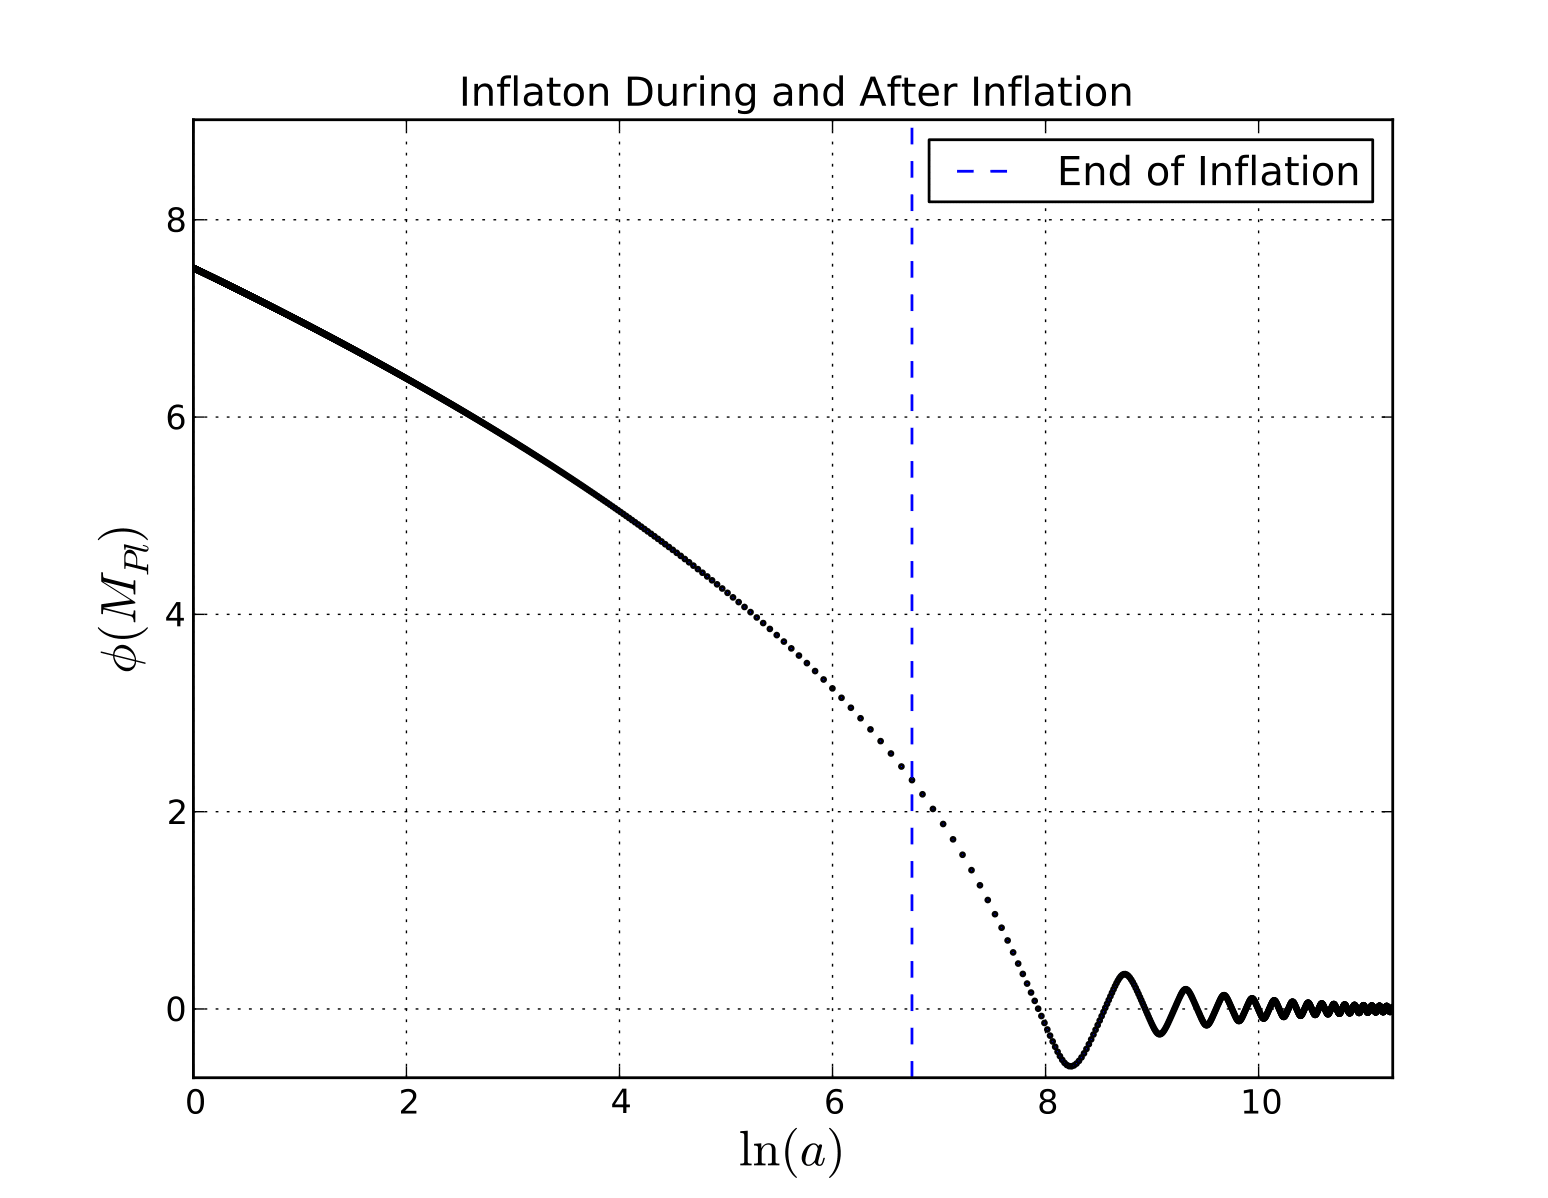
\includegraphics[width=0.75\textwidth]{inflaton_plot1.pdf}
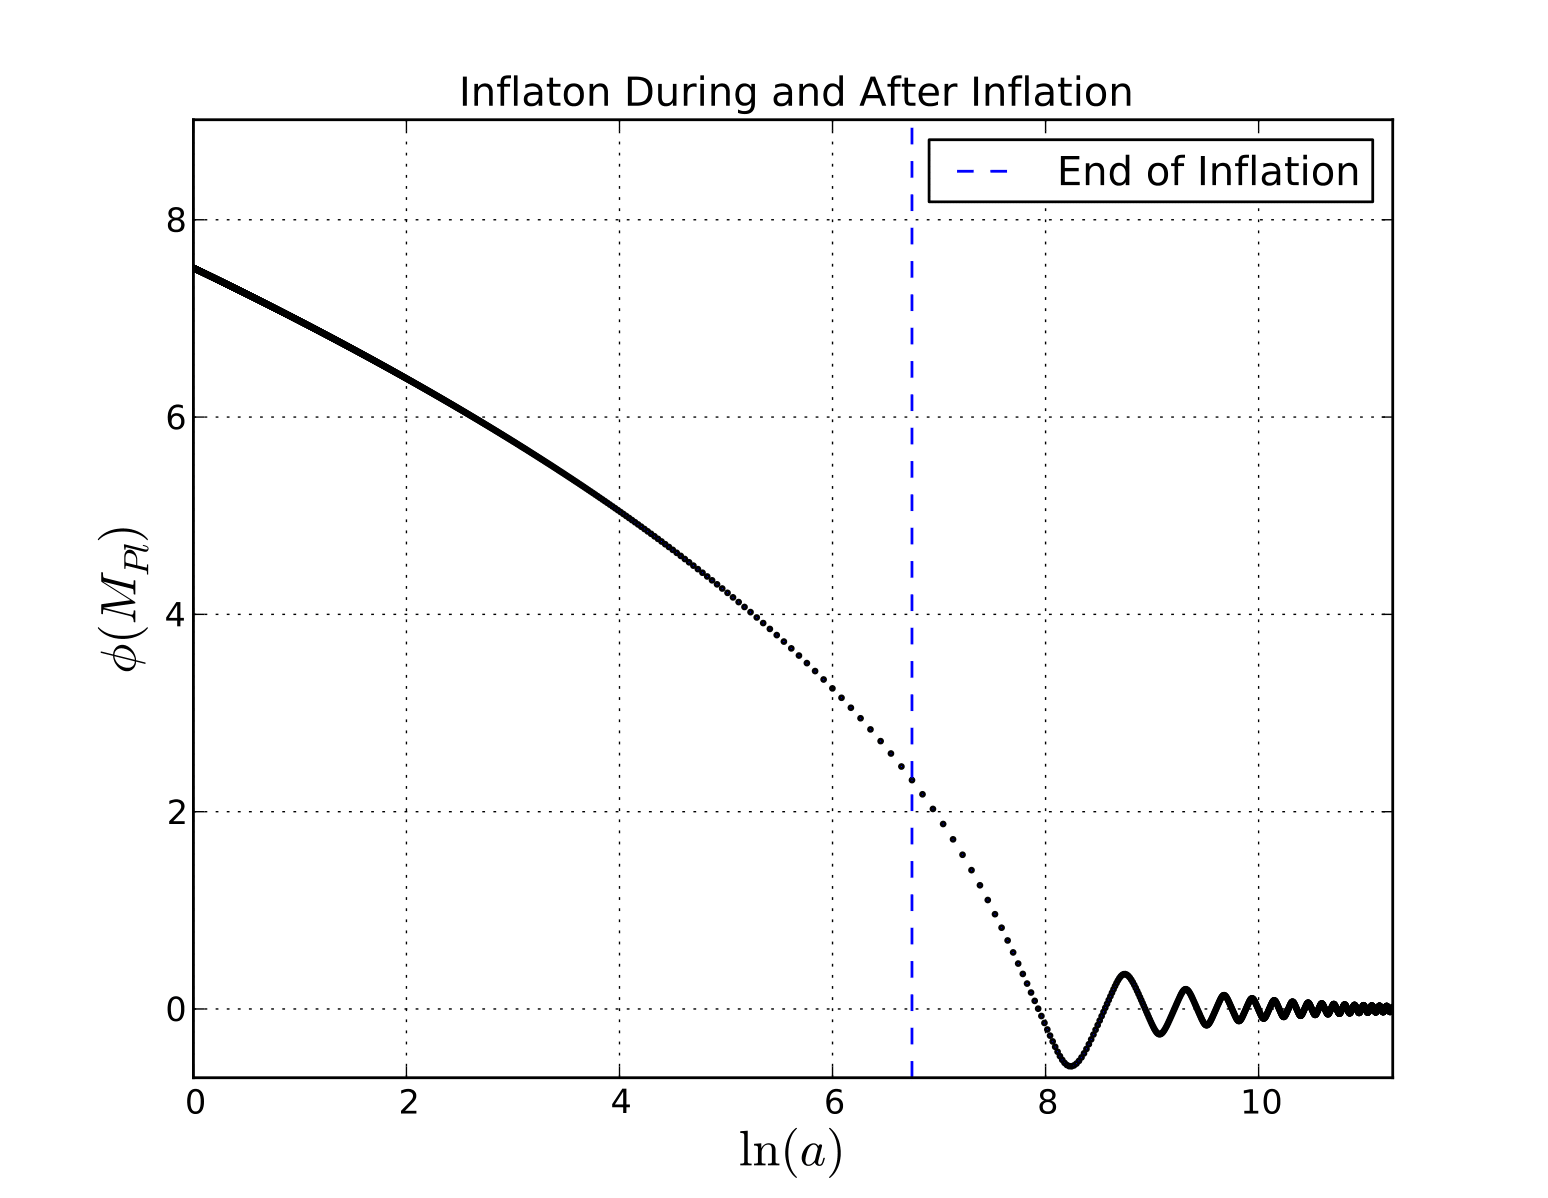
\includegraphics[width=0.75\textwidth]{inflaton_plot1.png}
\caption{Value of the inflaton field (in units of $M_{Pl}$) plotted against the logarithm of the scale factor in an inflationary model with a potential $V \sim \phi^4$, the dashed line marks the end of inflation. During inflation $\phi$ changes monotonically, sometime after the end of inflation the behaviour of $\phi$ becomes oscillatory.}
\label{inflation plot}
\end{center}
\end{figure}

For definiteness we will take $\phi>0$ at initial conditions, then noting that $\phi$ decreases monotonically during inflation (see Figure \ref{inflation plot}) $\phi$ can be thought of as a decreasing time-like variable during inflation. 

\subsection{The $\zeta$ Parameter} \label{zeta theory}
%Should talk about why production of entropy is important
In this section the $\zeta$ parameter is introduced as a way of tracking when the production of entropy occurs. To identify the production on entropy consider 
\begin{align}
\ud (\rho V) + P\ud V &= T \ud S \\
\ud \rho + (\rho + P)\ud(\mathrm{ln}V) &= \frac{T\ud S}{V}.
\end{align}
The time derivative of entropy within a comoving volume can now be calculated by rewriting the physical volume in terms of a constant comoving volume and the scale factor, $V=V_{comoving}a^3$,
\begin{equation}
\frac{T}{V}\frac{\ud S}{\ud t} = \dot{\rho} + 3(\rho + P)H. \label{S rate}
\end{equation}
An immediate consequence of the above equation, (\ref{S rate}), is that entropy within a comoving volume will be conserved so long as the fluid equation (\ref{fluid eqn}) holds. The situation in which (\ref{fluid eqn}) fails to hold is one in which there is is energy transfer between comoving volumes, such a situation requires some amount of inhomogeneity. This requirement for inhomogeneity links the non-conservation of $\zeta$ to the production of spatial gradients in the scalar fields.

With the intention of identifying when a change in entropy occurs we now define the $\zeta$ parameter \cite{pers} by its differential as
\begin{equation}
\ud \zeta \equiv \frac{\ud \mathrm{ln}\,\rho}{3(1+P/\rho)} + \ud\, \mathrm{ln} a.
\end{equation}
The time derivative of $\zeta$ is then given by
\begin{equation}
\frac{\ud \zeta}{\ud t} = \frac{1}{3(\rho + P)}\frac{\ud \rho}{\ud t} + H. \label{zeta rate}
\end{equation}
Equivalently in the case of scalar fields, using the energy density, pressure, and equation of motion for a scalar field, (\ref{rho eqn}), (\ref{p eqn}), and (\ref{eom phi}) respectively, allows (\ref{zeta rate}) to be rewritten as
\begin{equation}
\frac{\ud \zeta}{\ud t} = \sum_i \frac{\nabla \dot{\phi}_i \cdot \nabla \phi_i + \dot{\phi}_i\nabla^2\phi_i}{3a^2(\rho + P)}. \label{zeta source}
\end{equation}
The condition for the right-hand side of (\ref{zeta rate}) to be nonzero is exactly the condition that the right-hand side of (\ref{S rate}) also be nonzero, so $\zeta$ is conserved except during periods of entropy production.

If the evolution of the scalar fields and scale factor is known then (\ref{zeta source}) can be integrated to find $\zeta$ as a function of time, by convention $\zeta=0$ is chosen as the initial condition.

\section{Computation Techniques} \label{computation}
The equations of motion for a scalar field in an expanding universe are partial differential equations and are non-linear due to the dependence of the Hubble parameter $H$ on the scalar field and its derivatives and, in general, non-linear terms from $V_{,\phi_i}$. In this work the equations of motion are solved numerically using an as of yet unnamed lattice simulation code developed by Jonathan Braden \cite{latcode}. Using a lattice simulation to solve the equations of motion has the advantage that nonlinear effects are included in the calculation.

In order to solve the equations of motion (\ref{eom phi}) the system is recast into a Hamiltonian framework within the lattice simulation and space is evenly discretizes within a fixed comoving volume. A lattice site refers to a discrete point within the comoving volume being simulated, while the set of all lattice sites is referred to simply as the lattice. Values of scalar fields, $\phi_i$ and their momenta are stored for each lattice site with periodic boundary conditions imposed on the lattice. While the scalar fields are allowed to vary over the lattice, a flat FRW universe is assumed for the calculation of the scale factor, $a$, and the Hubble parameter, $H$, which are calculated uniformly over the lattice. The assumption that a FRW universe provides a good estimate for the evolution of spacetime can be physically motivated by the near homogeneity of the inflaton field during inflation.

The lattice simulation makes use of a pseudo-spectral method to calculate spacial derivatives, whereby a fast Fourier transform (FFT) is taken of the value to be differentiated over the lattice and the derivative calculated in Fourier space and finally the inverse FFT is used to return the derivatives to real space.

Initial conditions for the inflaton field and its momentum are chosen to have a mean value consistent with the slow-roll approximation $\ddot{\phi} \approx 0$. Fluctuations to the fields are added as a sampling of a Gaussian random field, the physical motivation for these field fluctuations is to provide one realization of the quantum fluctuations of the fields.

To the benefit of this work in investigating the effects of an instability during inflation, the lattice simulation code used is easily configurable to change the potential being considered. By running the lattice simulation twice from identical initial conditions and fluctuations, once with an instability in the potential and once without, the effects of the instability can be isolated by comparing between the two runs.
%The equations of motion for a scalar field in an expanding universe are partial differential equations and are non-linear due to the dependence of the Hubble parameter $H$ on the scalar field and its derivatives and, in general, non-linear terms from $V_{,\phi_i}$. In this work the equations of motion are solved numerically using a lattice simulation code developed by Jonathan Braden. Using a lattice simulation to solve the equations of motion has the advantage that nonlinear effects are included in the calculation.

%In the lattice simulation used 

%The advantage of using the lattice simulation is the ability to keep track of any nonlinearities that may arise, while the specific code used makes use of an accurate integration scheme and is capable of producing numerically accurate results. %this is a statement that should be supported

%In the lattice simulation, while the scalar fields are allowed to vary across the lattice, a flat FRW universe is assumed for the calculation of the scale factor, $a$, and Hubble parameter, $H$. The assumption of a FRW universe provides a good estimate for the evolution of spacetime can be physically motivated by the near homogeneity of the inflaton field.

%The lattice simulation solves for the evolution of a number of scalar fields from initial conditions as well as solving for the scale factor and Hubble factor assuming a FRW metric. For each site on the lattice values of the matter fields are stored, whereas the scale factor and Hubble parameter are assumed to be uniform over the simulation box. Derivative terms are calculated using a pseudo spectral method whereby a fast Fourier transform (FFT) is taken of the matter field values over the simulation box, then derivatives are then calculated in Fourier and finally the FFT is inverted to return the derivatives to real space.

%The equations of motion are cast into a Hamiltonian framework and the resulting system of equations discretized so that each point of the lattice is associated with its own conjugate variables. We have from Hamiltonian mechanic

%The system of equations so discretized , Hamilton's equations are put into a matrix equation format and finding the solutions to the equations of motion is equivalent to integrating this matrix equation.

\section{Transverse Instability in the Two Field Model} \label{two field}

%This makes sense for the start of this section
%In what follows, we will consider an extension to the above single field inflationary scenario by including a second scalar field, $\chi$. In the case we consider inflation is driven by the $\phi$ field (termed longitudinal), while the  $\chi$ field (termed transverse) is composed of fluctuations around zero. The specific scenario being considered is one in which as inflation proceeds along the longitudinal direction an instability develops in the transverse direction and persists for a finite time. The potential considered is,

In what follows, we will consider an extension to the single field inflationary scenario described above by including a second scalar field, $\chi$, which is initialized with small fluctuations around the minimum of its potential. Inflation is still driven by the field $\phi$ while additional dynamics are associated with the field $\chi$, the terminology is that $\phi$ is the longitudinal field while $\chi$ is the transverse field. The specific scenario considered is one in which as inflation proceeds in the longitudinal direction the potential changes shape so as to create an instability in the transverse direction, this instability is transient and as inflation continues in the longitudinal direction the transverse instability is removed and the potential returns to its original form.

%Should say here what effects are of interest ie. what remains after the potential has returned to its original form

\subsection{The Two Field Potential}
The specific form of potential chosen to explore the above scenario is
\begin{equation}
V(\phi, \chi) = \frac{\lambda_{\phi}}{4}\phi^4 + \frac{\lambda_{\chi}}{4}\chi^4 + \Delta V(\phi, \chi), \label{potential}
\end{equation}
where $\Delta V$ provides the transient instability in the transverse direction. The form chosen for $\Delta V$ is given by
\begin{equation}
\Delta V = -\frac{A^2\sqrt{e}}{b}(\phi - \phi_p)\mathrm{exp}\bigg[-\frac{(\phi-\phi_p)^2}{2b^2}\bigg]\chi^2. \label{dv}
\end{equation}
The parameters $A^2$, $b$, and $\phi_p$ respectively control the magnitude, width, and placement along the longitudinal direction of $\Delta V$, the overall sign convention for $\Delta V$ is a result of having chosen the convention that $\phi>0$ during inflation. It can be noted that this form of $\Delta V$ is an effective mass term for the $\chi$ field. When $|\phi-\phi_p| \gg, b$ $\Delta V \approx 0$ and has negligible effect. As $\phi$ approaches $\phi_p$ from above the $\chi$ field acquires a negative effective mass squared which reaches a minimum at $\phi = \phi_p + b$ (the potential remaining bounded from below by the $\chi^4$ term in (\ref{potential})). Likewise, as $\phi$ approaches $\phi_p$ from below the $\chi$ field acquires a positive effective mass squared which reaches a maximum at $\phi = \phi_p - b$. The surface of this potential is shown in Figure \ref{potential plot} while the effective mass of $\chi$ is shown in Figure \ref{meff2 plot}.

\begin{figure}
\begin{center}
%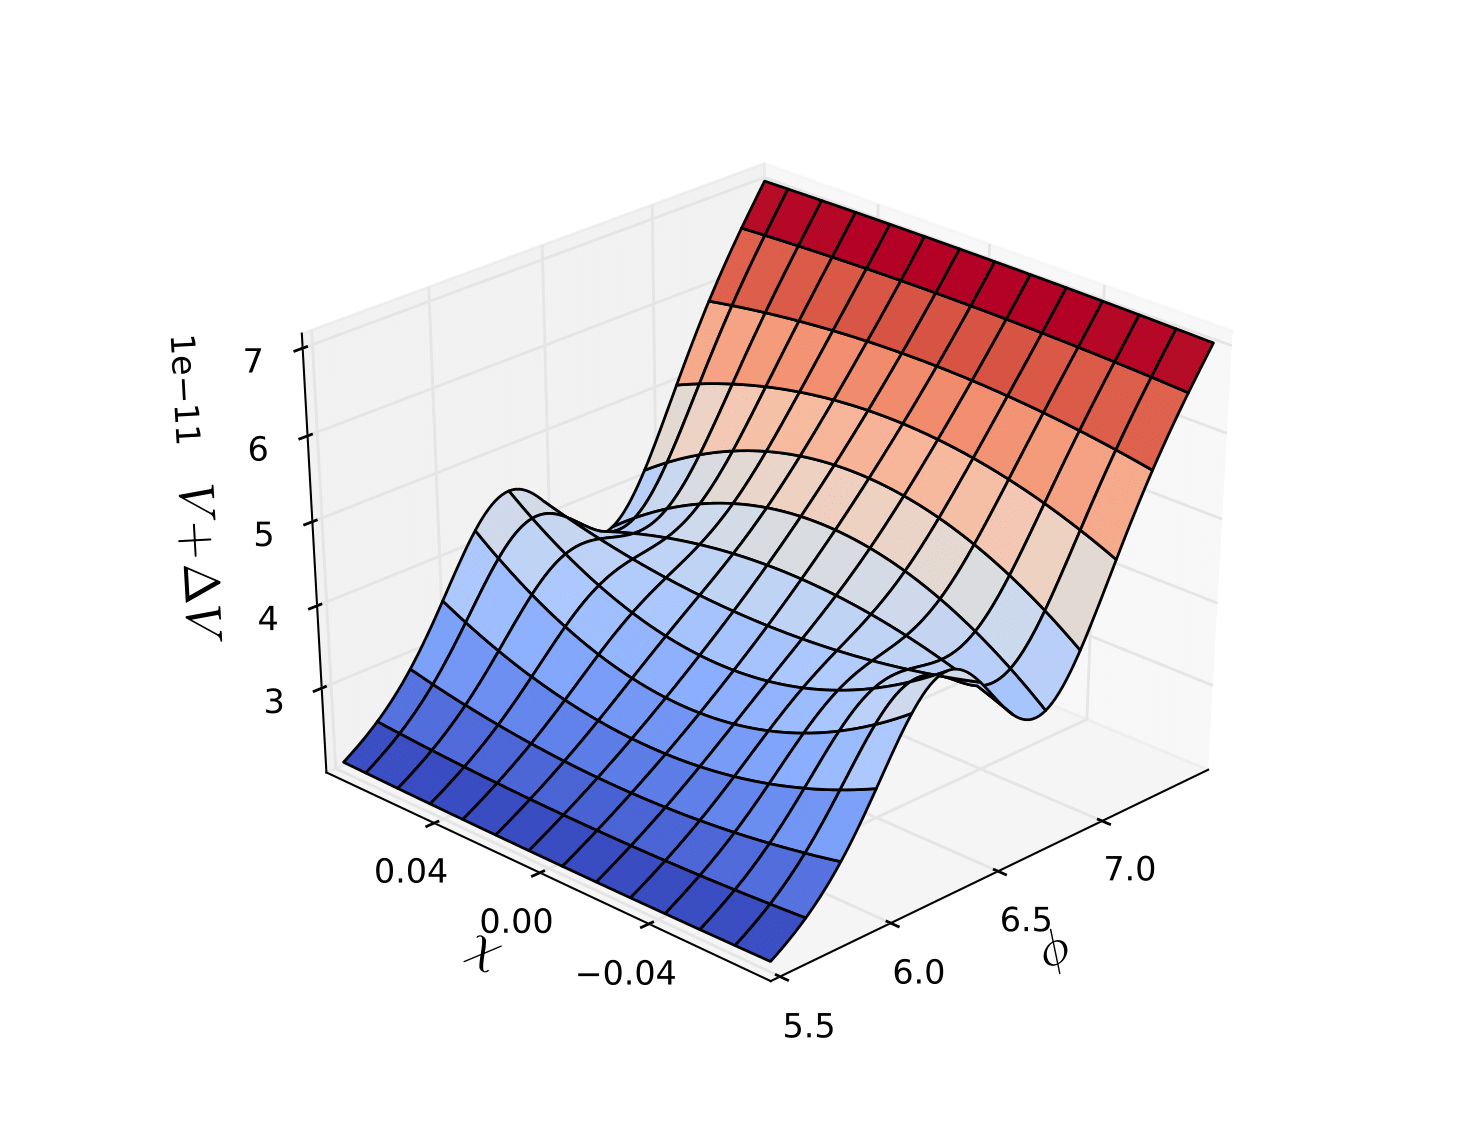
\includegraphics[width=0.75\textwidth]{potential_plot1.pdf}
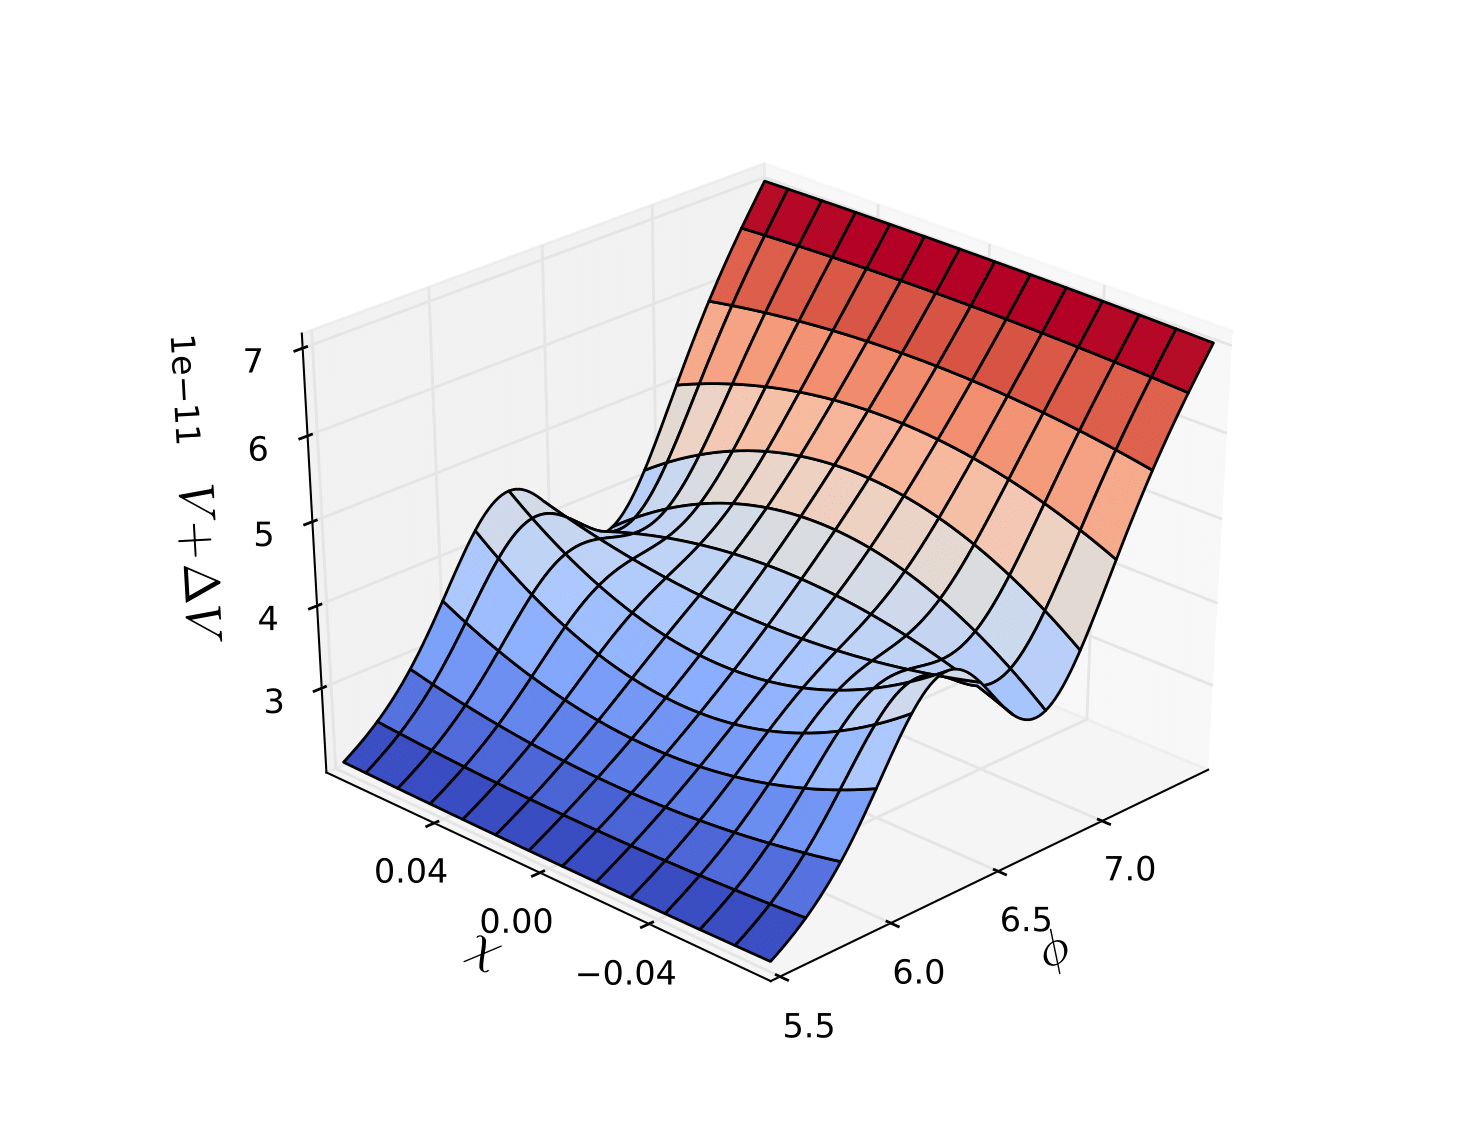
\includegraphics[width=0.75\textwidth]{potential_plot1.png}
\caption{An example potential surface in the form of (\ref{potential}). The transverse instability is visible as the portion of the potential surface which is concave down along the $\chi$ direction, $\chi=0$ becomes stable for the portion of the potential surface that is concave up along the $\chi$ direction. The overall downwards slope from larger to lower values of $\phi$ is due to the $\phi^4$ term in the potential and is mainly responsible for driving inflation in the longitudinal direction. Fields are in units of $M_{Pl}$.}
\label{potential plot}
\end{center}
\end{figure}

\begin{figure}
\begin{center}
%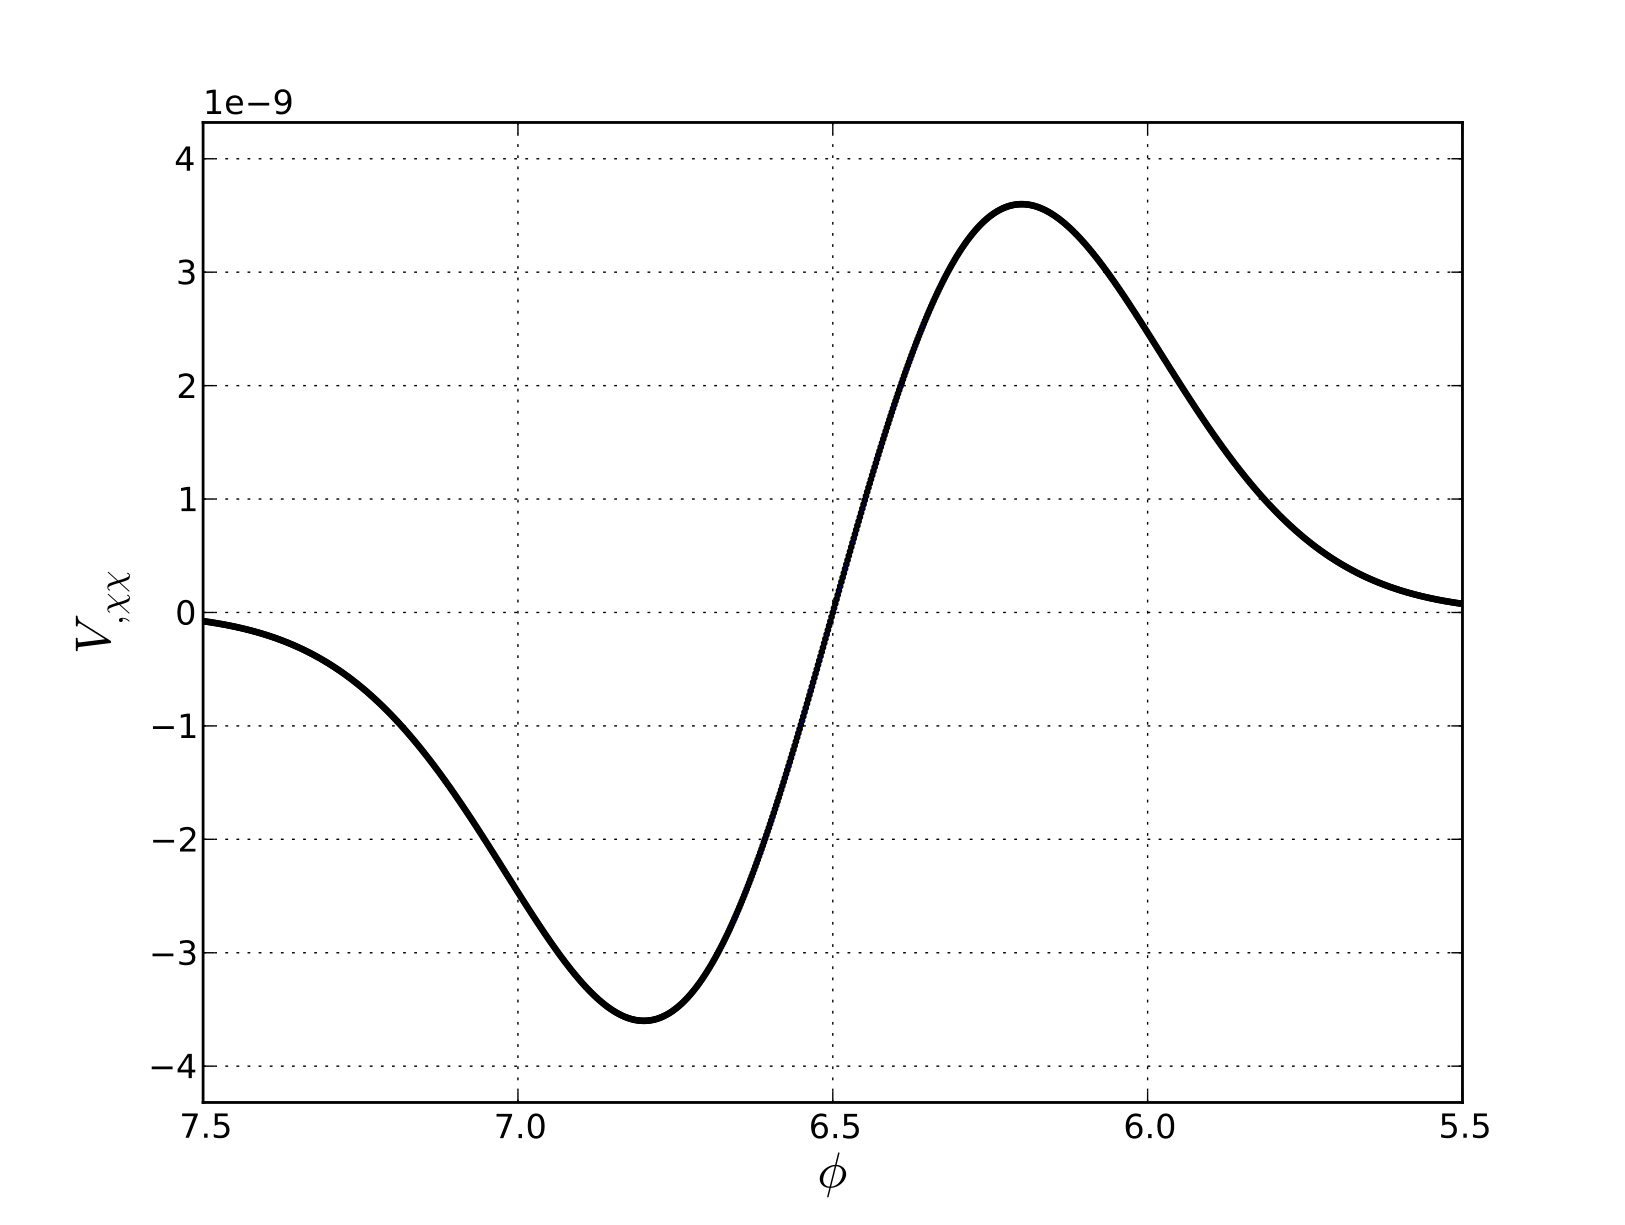
\includegraphics[width=0.75\textwidth]{meff2_plot.pdf}
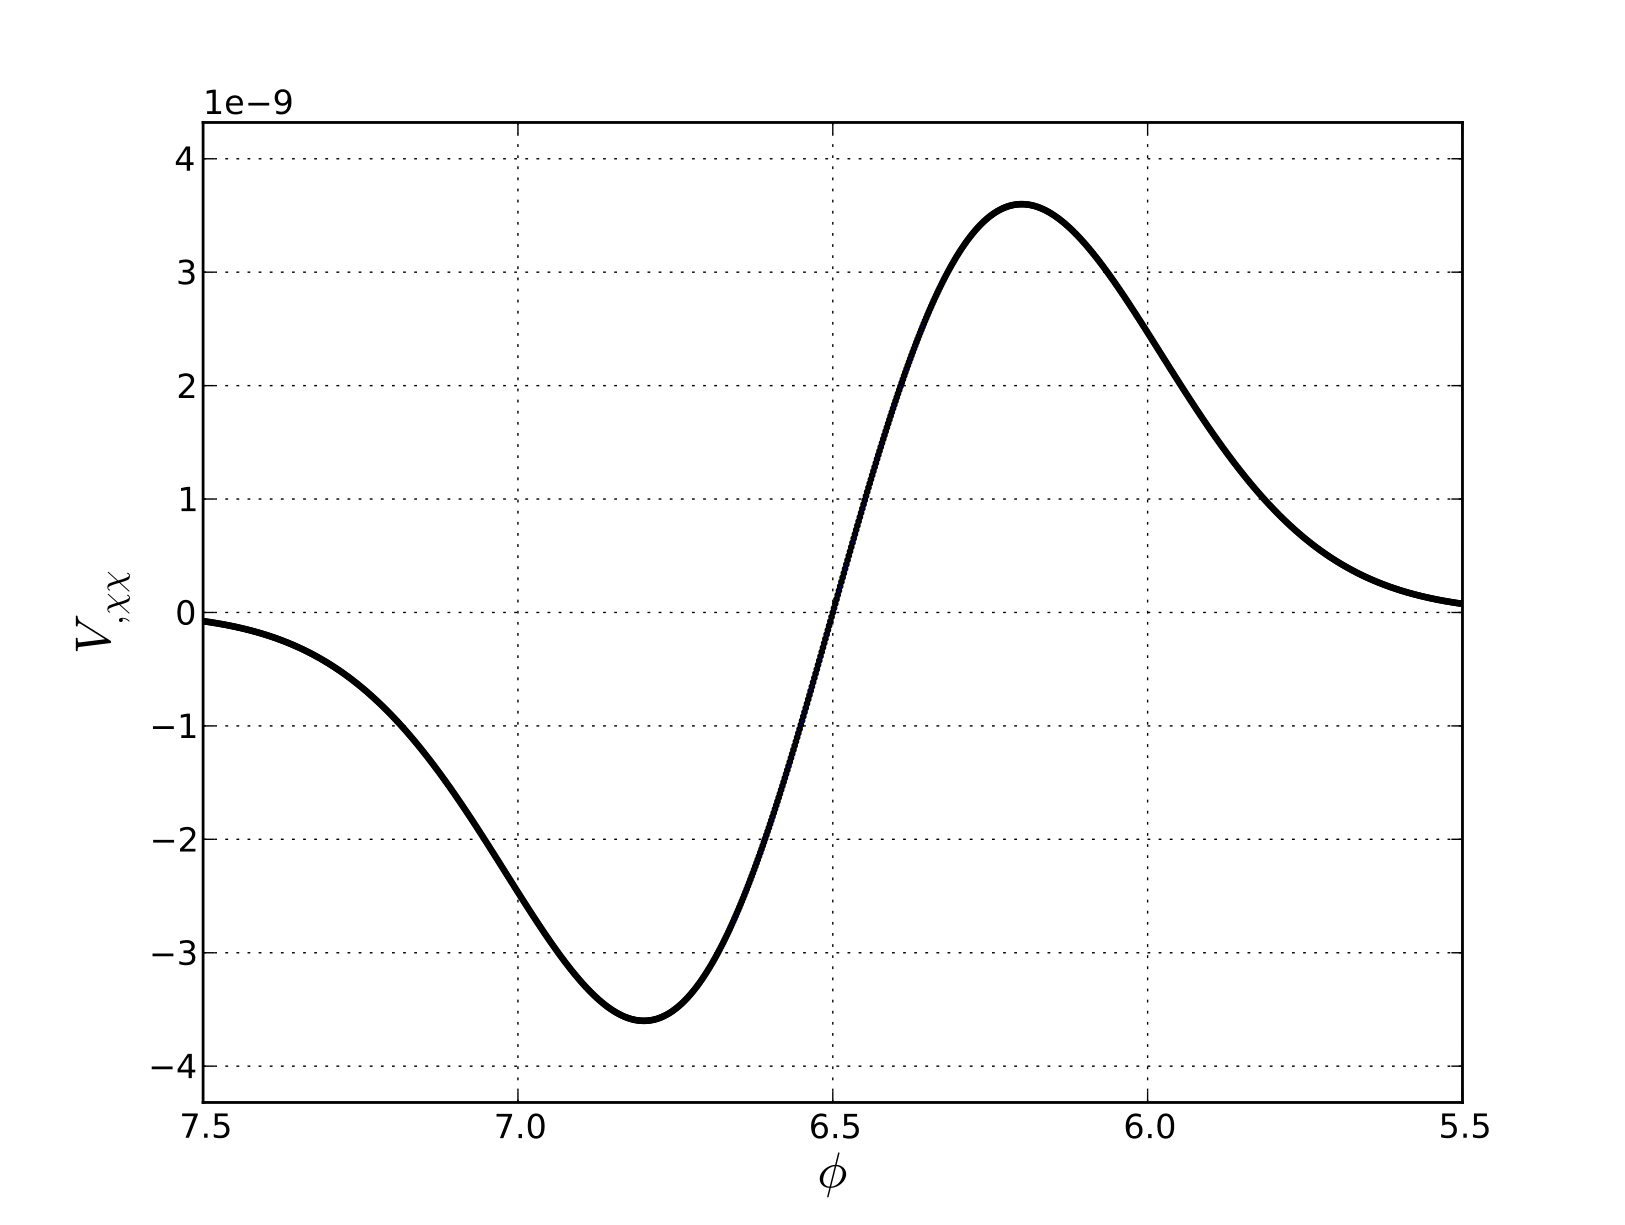
\includegraphics[width=0.75\textwidth]{meff2_plot.png}
\caption{A visualization of the transverse instability, the effective mass squared of $\chi$ (evaluated along $\chi=0$ with parameters $b=0.3M_{Pl}$, $\phi_p=6.5M_{Pl}$). For $\phi>\phi_p$ the transverse field is unstable around $\chi=0$, for $\phi<\phi_p$ the transverse field becomes stable around $\chi=0$. This plot relates to the potential surface in Figure \ref{potential plot} by being a measure of its curvature in the $\chi$ direction.}
\label{meff2 plot}
\end{center}
\end{figure}

With the inclusion of a nonzero $\Delta V$ in (\ref{potential}) there is, associated with the instability in the transverse direction, a change in $V_{,\phi}$ which becomes more significant as $\chi$ is driven away from zero
\begin{equation}
V_{,\phi} = \lambda_{\phi}\phi^3 - \frac{A^2\sqrt{e}}{b}\bigg(1 - \frac{(\phi-\phi_p)^2}{b^2}\bigg)\mathrm{exp}\bigg[-\frac{(\phi-\phi_p)^2}{2b^2}\bigg]\chi^2. \label{dv phi}
\end{equation}
There is then the possibility that applying a transverse instability of the form (\ref{dv}) will significantly alter the evolution of the longitudinal field, potentially causing an early end to inflation. As the target of investigation for the current work is one in which inflation continues along the longitudinal direction it will be necessary to place appropriate bounds on the potential considered (the case where $V_{,\phi}$ changes sufficiently to stop $\phi$ from proceeding towards zero is a realization of the trpping mechanism, but not the subject of this report \cite{kofman}).

If we wish to consider the case that inflation continues during the transverse instability we should require $\dot{\phi}<0$ during inflation, that is $\phi$ continues to roll down its potential without reversing direction. In order to remain consistent with this requirement for inflation to continue we impose a set of bounds on the parameters of $\Delta V$. To estimate this set of bounds, note that in the slow-roll approximation the requirement $\dot{\phi}<0$ is equivalent to $V_{,\phi}>0$. In the slow-roll approximation it is sufficient to require that over the range of values of $\phi$ and $\chi$ covered during the evolution of the system $V(\phi, \chi)$ does not attain a local maximum. It is in principle possible to solve for this condition numerically, however by making several approximations a sufficient condition can be derived.
%Can related this part to the trapping mechanism

The domain of interest, where inflation along the longitudinal direction could be stopped by the addition of $\Delta V$ to the potential is the region where $\Delta V_{,\phi} < 0$, from (\ref{dv phi}) this is $|\phi - \phi_p|<b$. The inclusion of the $\chi^4$ term in the potential insures that the range of $\chi$ remains bounded, let $|\chi|_{max}$ be a bounding value on $\chi$ so that $|\chi| \leq |\chi|_{max}$. Within the range $|\phi-\phi_p|<b$ and $|\chi|<|\chi|_{max}$ a lower bound can be placed on $\Delta V_{,\phi}$, comparing to (\ref{dv phi}) we have
\begin{align}
\Delta V_{,\phi}(\phi, \chi) &\geq \Delta V_{,\phi}(\phi=\phi_p, \chi=|\chi|_{max}) \\
&= -\frac{A^2\sqrt{e}}{b}|\chi|_{max}^2.
\end{align}
The above bound on $\Delta V_{,\phi}$ leads to a lower bound on $V_{,\phi}$ for values of $\phi$ and $\chi$ in the stated range,
\begin{align}
V_{,\phi}(|\phi-\phi_p|<b, |\chi|<|\chi|_{max}) \geq \lambda_{\phi}(\phi_p-b)^3 - \frac{A^2\sqrt{e}}{b}|\chi|_{max}^2.
\end{align}
Then in the same range and in the slow-roll approximation a sufficient condition to insure that inflation along the longitudinal direction is not stopped by including the $\Delta V$ term in the potential is given by
\begin{equation}
\frac{\lambda_{\phi}(\phi_p-b)^3b}{\sqrt{e}A^2} \geq |\chi|_{max}^2. \label{param bound}
\end{equation}

It should be noted that $|\chi|_{max}$ is also determined by the potential parameters and the initial magnitude of $\chi$ fluctuations, so the bound on potential parameters provided by (\ref{param bound}) is incomplete. In principle $|\chi|_{max}$ can be estimated from the parameters of the potentials, however even without performing such an estimate (\ref{param bound}) can still be used a scaling relation for the maximum effect size the transverse instability can provide while still allowing inflation to continue along the longitudinal direction.

%\begin{align}
%V_{,\phi}(\phi=\phi_p, \chi=|\chi|_{max} & \leq 0 \\
%\lambda_{\phi}\phi^3 - \frac{A^2\sqrt{e}}{b}|\chi|^2_{max} & \leq 0\\
%\frac{b\lambda_{\phi}}{A^2\sqrt{e}}\phi_p^3 \leq |\chi|^2_{max}
%\end{align}


%There is associated with the instability in $\chi$ caused by $\Delta V$ an instability in $\phi$ and if we wish to use $\phi$ as a time-like variable during inflation it should be verified that it remains monotonic for cases with non-zero $\Delta V$. Although it is possible to violate the monotonicity with a large enough $\Delta V$, in practice the monotonicity condition is easy to satisfy due to our choice of $\phi$ as longitudinal and $\chi$ as transverse. This choice means that during inflation $|\phi| \gg |\chi|$ will be satisfied and the sign of $V_{\phi}$ will not change for small enough $\Delta V$.

%The effect of a nonzero $\Delta V$ in the potential is that $\chi$ will experience a temporary tachyonic instability as $\phi$ passes through the point $\phi=\phi_p$ while driving inflation. During this instability the $\chi$ field will experience exponential growth away from zero, with points where the fluctuations of $\chi$ are positive will exponentially increase, while points where the fluctuations of $\chi$ are negative will exponentially become more negative. The net effect of this instability is to cause a separation between trajectories of initially similar fluctuations in $\chi$. As $\phi$ decrease below $\phi_p$ the instability is terminated and the separation of adjacent trajectories ceases. 

\subsection{Effects of Nonzero $\Delta V$}
The effect of introducing a nonzero $\Delta V$ term in the form of (\ref{dv}) to the potential is that as inflation proceeds in the longitudinal direction and $\phi$ decrease, $\chi$ will experience a transient tachyonic instability for values of $\phi \approx \phi_p+b \pm b$. As the transverse field, $\chi$, initially has a mean of zero the fluctuations of $\chi$ will take on both positive and negative values. During the instability positive fluctuations of $\chi$ will grow exponentially more positive, while negative fluctuations will grow exponentially more negative. The net effect of this instability is to cause a separation between trajectories of initially similar fluctuations in $\chi$, increasing the importance of gradient terms in the equations of motion. Once $\phi$ has decreased so that $\phi \leq \phi_p$ the transverse instability terminates and the $\Delta V$ term in the potential instead bestows $\chi$ with an effective mass, causing the field to oscillate with time for $\phi \approx \phi_p-b \pm b$. These oscillations are damped by the Hubble drag term in the equations of motion. This separation of trajectories is illustrated in Figure \ref{chi dv plot} which compares the evolution of the $\chi$ field sampled at different lattice sites as calculated with the inclusion of a $\Delta V$ term in the potential.

To examine, in more detail, the behaviour of $\chi$ after the transverse instability has terminated we can write down its equation of motion from (\ref{eom phi}), (\ref{potential}) and (\ref{dv})
\begin{align}
0 &= \ddot{\chi} + 3H\dot{\chi} + (-\frac{\Delta \chi}{a^2} + \lambda_{\chi}\chi^3 + \Delta V_{,\chi})\\
0 &= \ddot{\chi} + 3H\dot{\chi} + (-\frac{\Delta}{a^2} + \Delta V_{,\chi \chi})\chi + \lambda_{\chi}\chi^3. \label{eom chi}
\end{align} 
%For $\Delta V_{,\chi \chi}>0$ this is an oscillator equation with time dependent parameters, with anharmonicities arising due to the $\lambda_{\chi}\chi^3$ term and the indirect $\chi$ dependence of $\Delta V_{,\chi \chi}$ from coupling between $\phi$ and $\chi$. In analogy with an oscillator equation a restoring force is supplied by $\Delta V_{,\chi \chi}$ and Laplacian terms of $\chi$, damping is provided by the Hubble drag term. The effective mass term, $\Delta V_{,\chi \chi}$ becomes suppressed as $\phi$ decreases below $\phi_p-b$, the Laplacian term becomes suppressed as $a$ increases.
For $\Delta V_{,\chi \chi}>0$ this equation resembles a damped oscillator equation with time dependent parameters, and anharmonicities arising due to the $\lambda_{\chi}\chi^3$ term and the indirect $\chi$ dependence of $\Delta V_{,\chi \chi}$ from coupling between $\phi$ and $\chi$ . The qualitative behaviour of $\chi$ after the transverse instability can be explained assuming that the time dependence of the parameters in (\ref{eom chi}) vary slowly enough that treating (\ref{eom chi}) as a damped oscillator equation is a good approximation over short enough periods of time. If this is the case, then in analogy with a damped oscillator an effective restoring force is supplied by $\Delta V_{,\chi \chi}$ and Laplacian terms of $\chi$, with damping being provided by the Hubble drag term.

\begin{figure}
\begin{center}
%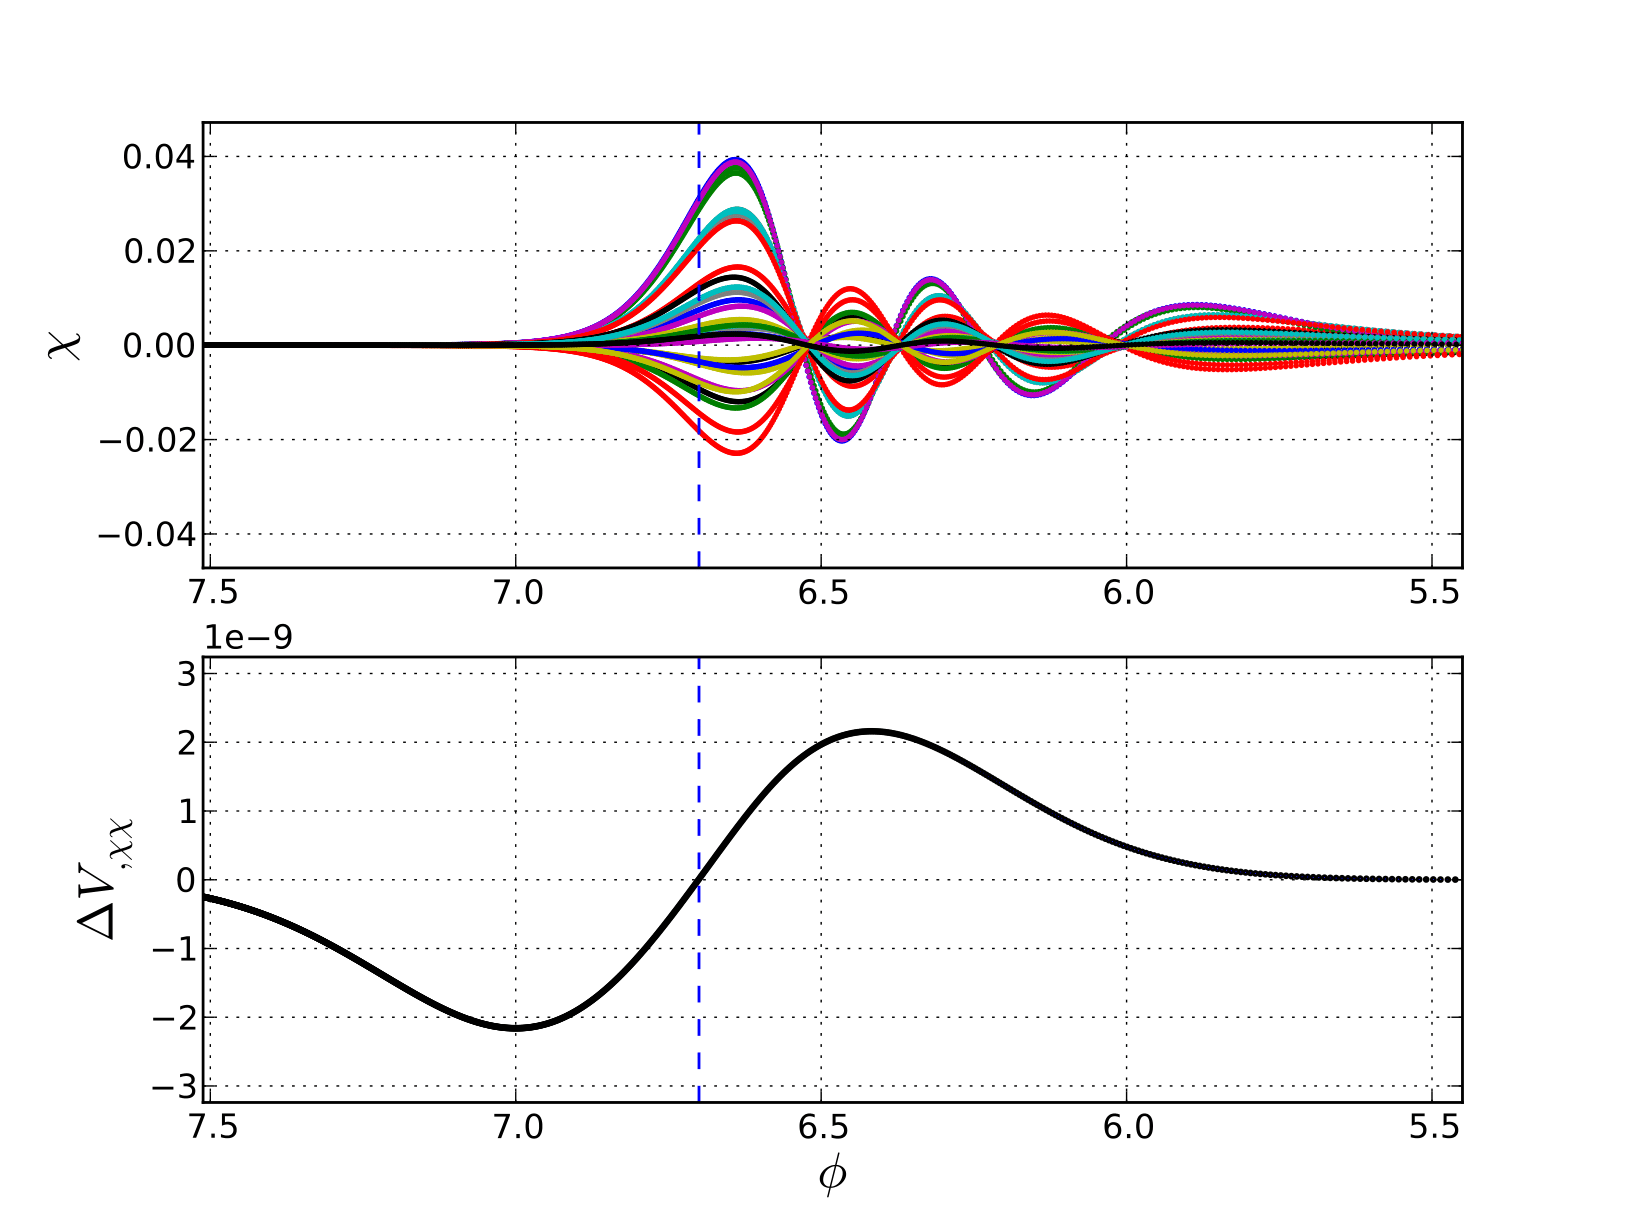
\includegraphics[width=0.75\textwidth]{chi_deltav_plot1.pdf}
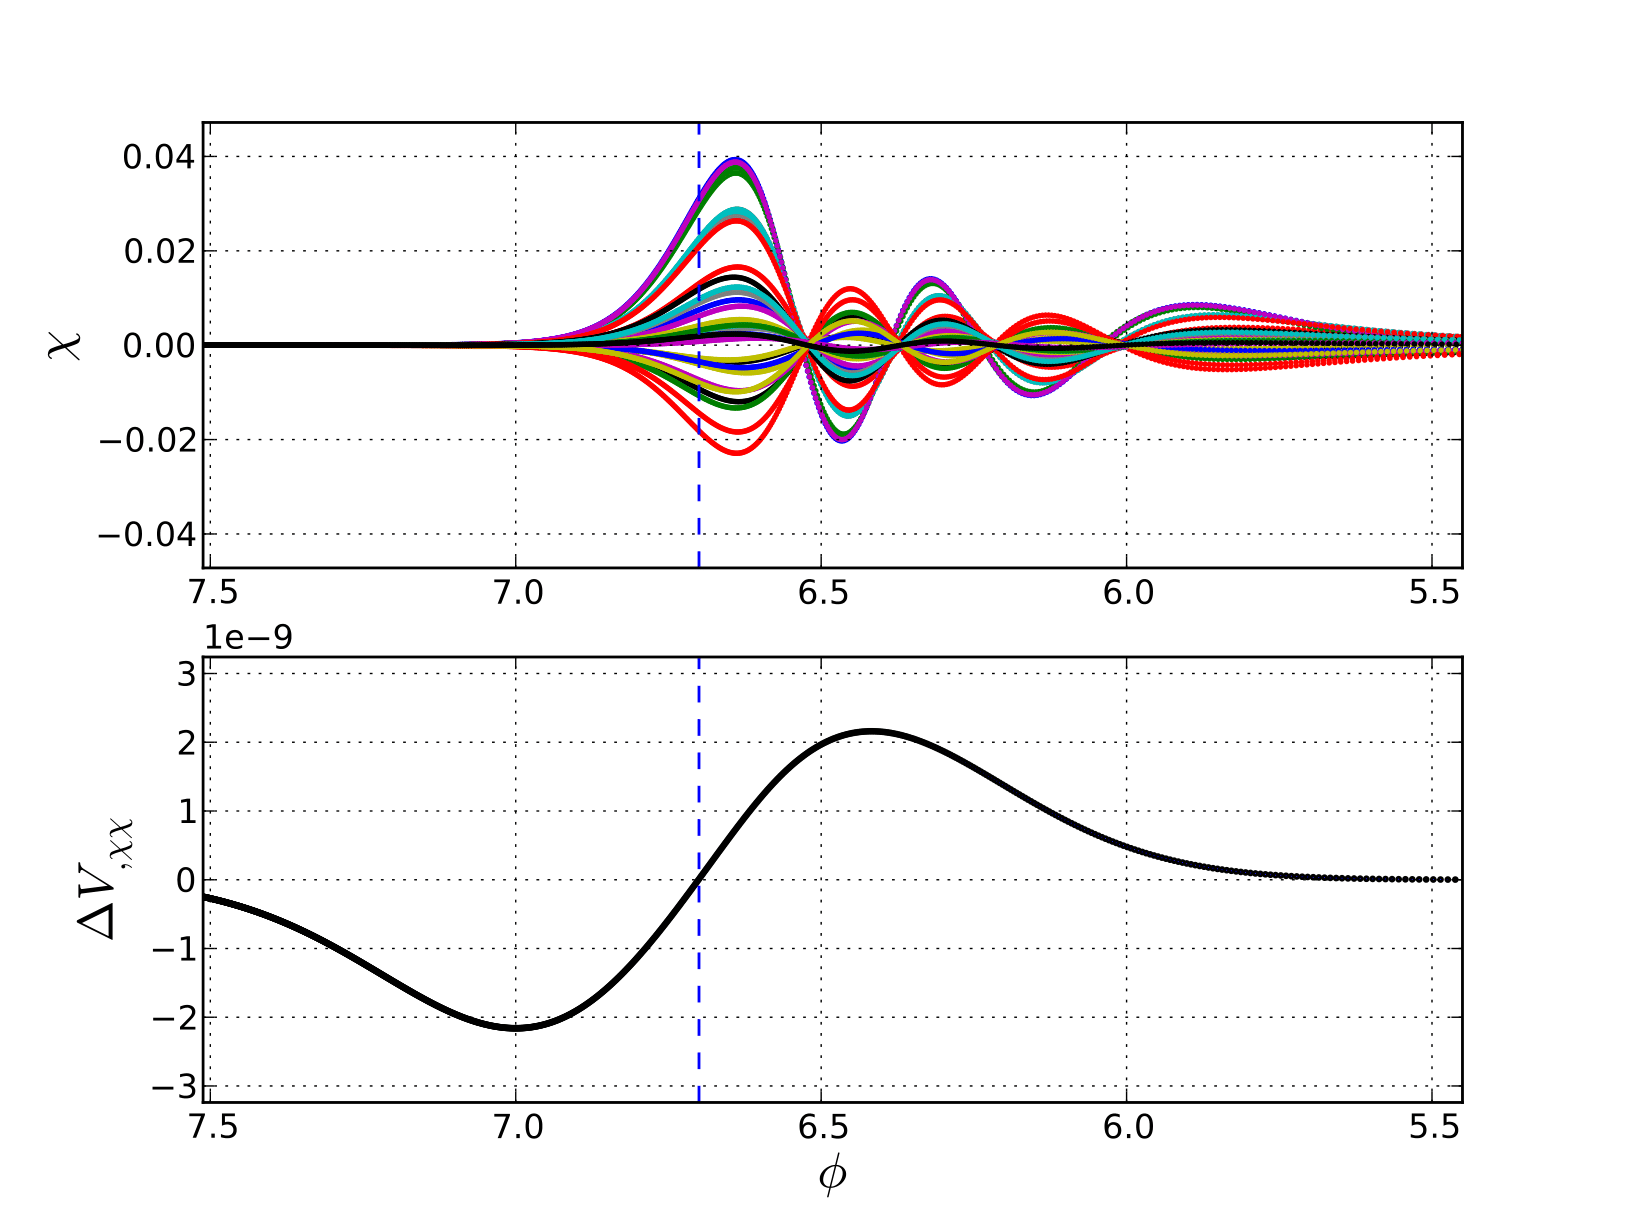
\includegraphics[width=0.75\textwidth]{chi_deltav_plot1.png}
\caption{\emph{Top:} The evolution of $\chi$ at sampled lattice points showing the effects of $\Delta V$. \emph{Bottom:} $\Delta V_{,\chi \chi}$ is a measure of the transverse instability, it is plotted here for the parameters of $\Delta V$ used in is the calculation of $\chi$ shown in the top plot.\\
The vertical dashed line is located at $\phi=\phi_p$, where the transverse direction transitions from unstable to stable. For $\phi>\phi_p$ trajectories of $\chi$ separate due to the transverse instability causing growth of fluctuations,  initial fluctuations in the $\chi$ field are smaller than the scale visible on this plot. For $\phi<\phi_p$ the transverse direction is stable and the $\chi$ field oscillates. Fields are units of $M_{Pl}$, $\Delta V_{,\chi \chi}$ is in units of $M_{Pl}^2$.}
\label{chi dv plot}
\end{center}
\end{figure}

With both sources of the effective restoring force becoming exponentially suppressed ($\Delta V_{,\chi \chi}$ due to the Gaussian tail for $\phi<\phi_p-b$ and $-\Delta/a^2$ due to the approximately exponential growth of $a$ during inflation) and the drag term $H$ only slowly varying during inflation the behaviour of the $\chi$ field will at some point change over from an oscillatory to an overdamped state. At some point after $\chi$ begins exhibiting overdamped behaviour the effective restoring force will become negligible and the field $\chi$ will approach a constant comoving configuration for the duration of inflation, this can be seen in Figure \ref{chi dv plot}.

%Talk about the two possibilities of what happens with respect to the restoring by gradient terms

\begin{figure}
\begin{center}
%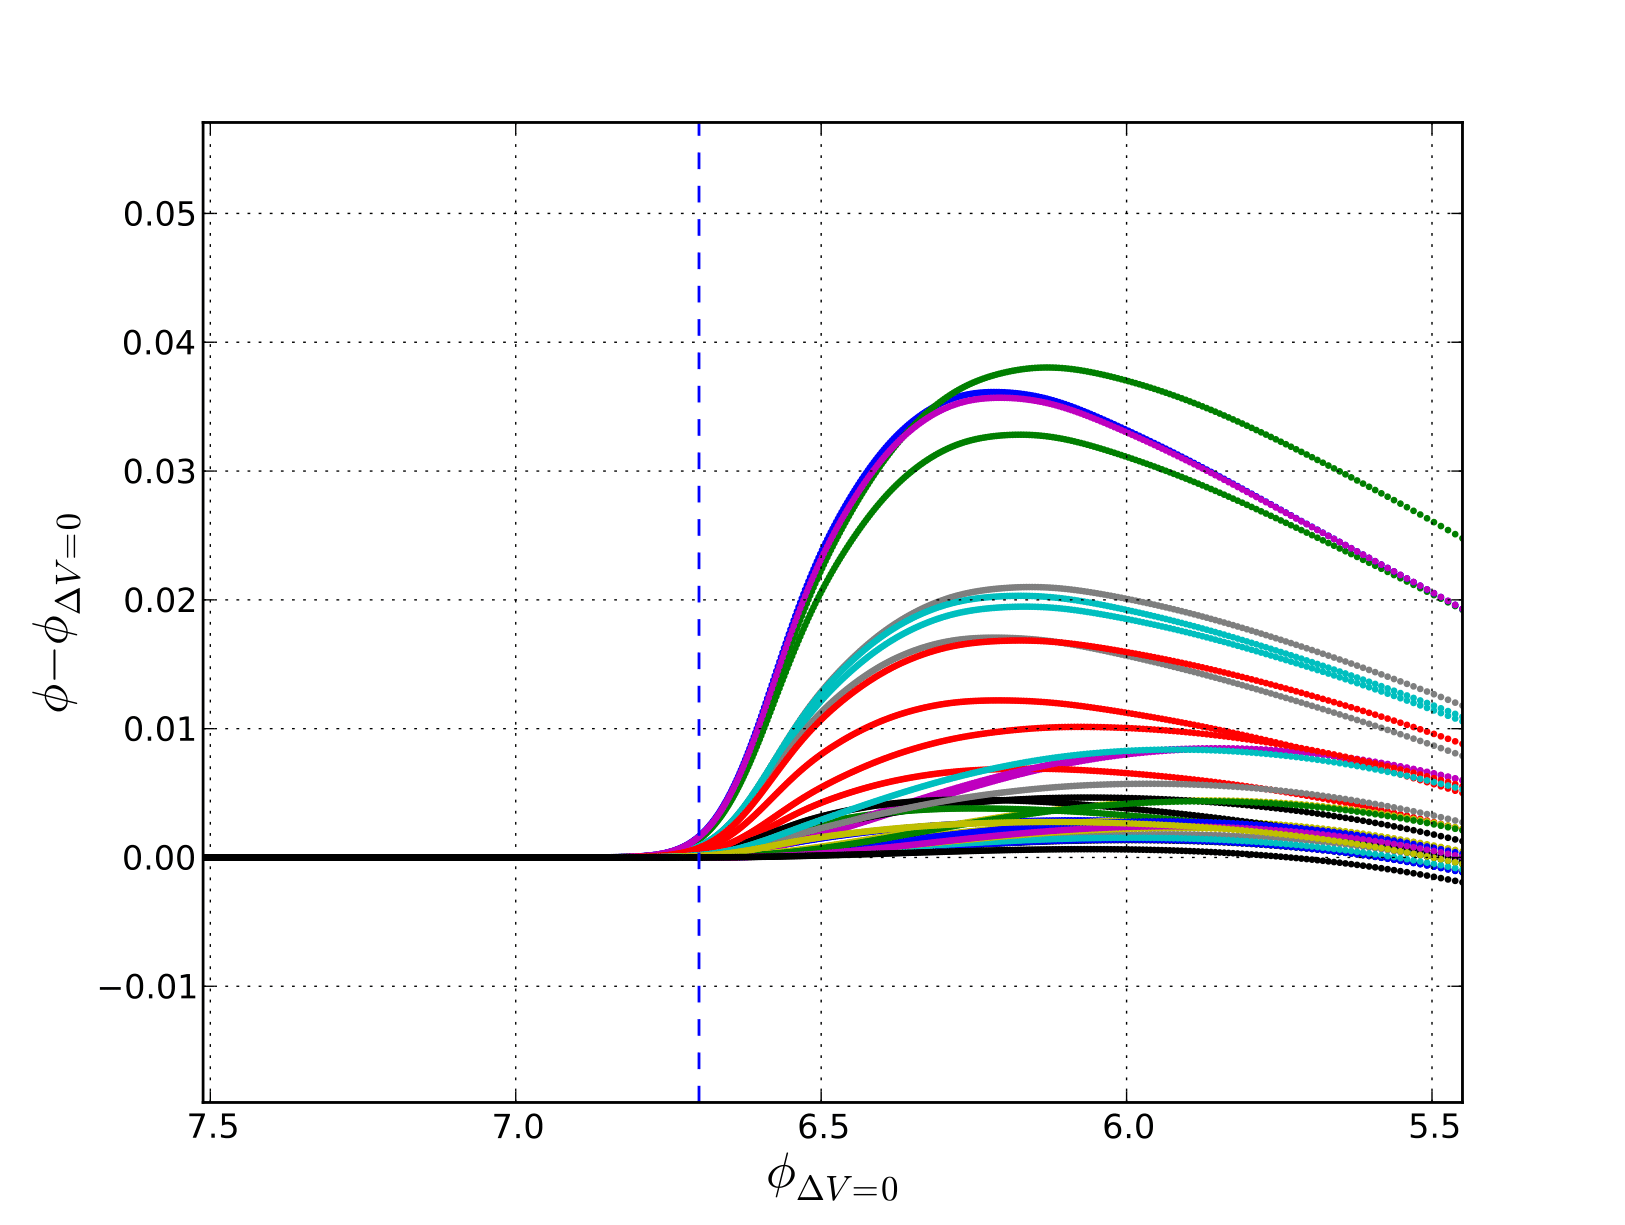
\includegraphics[width=0.75\textwidth]{phi_dif_plot.pdf}
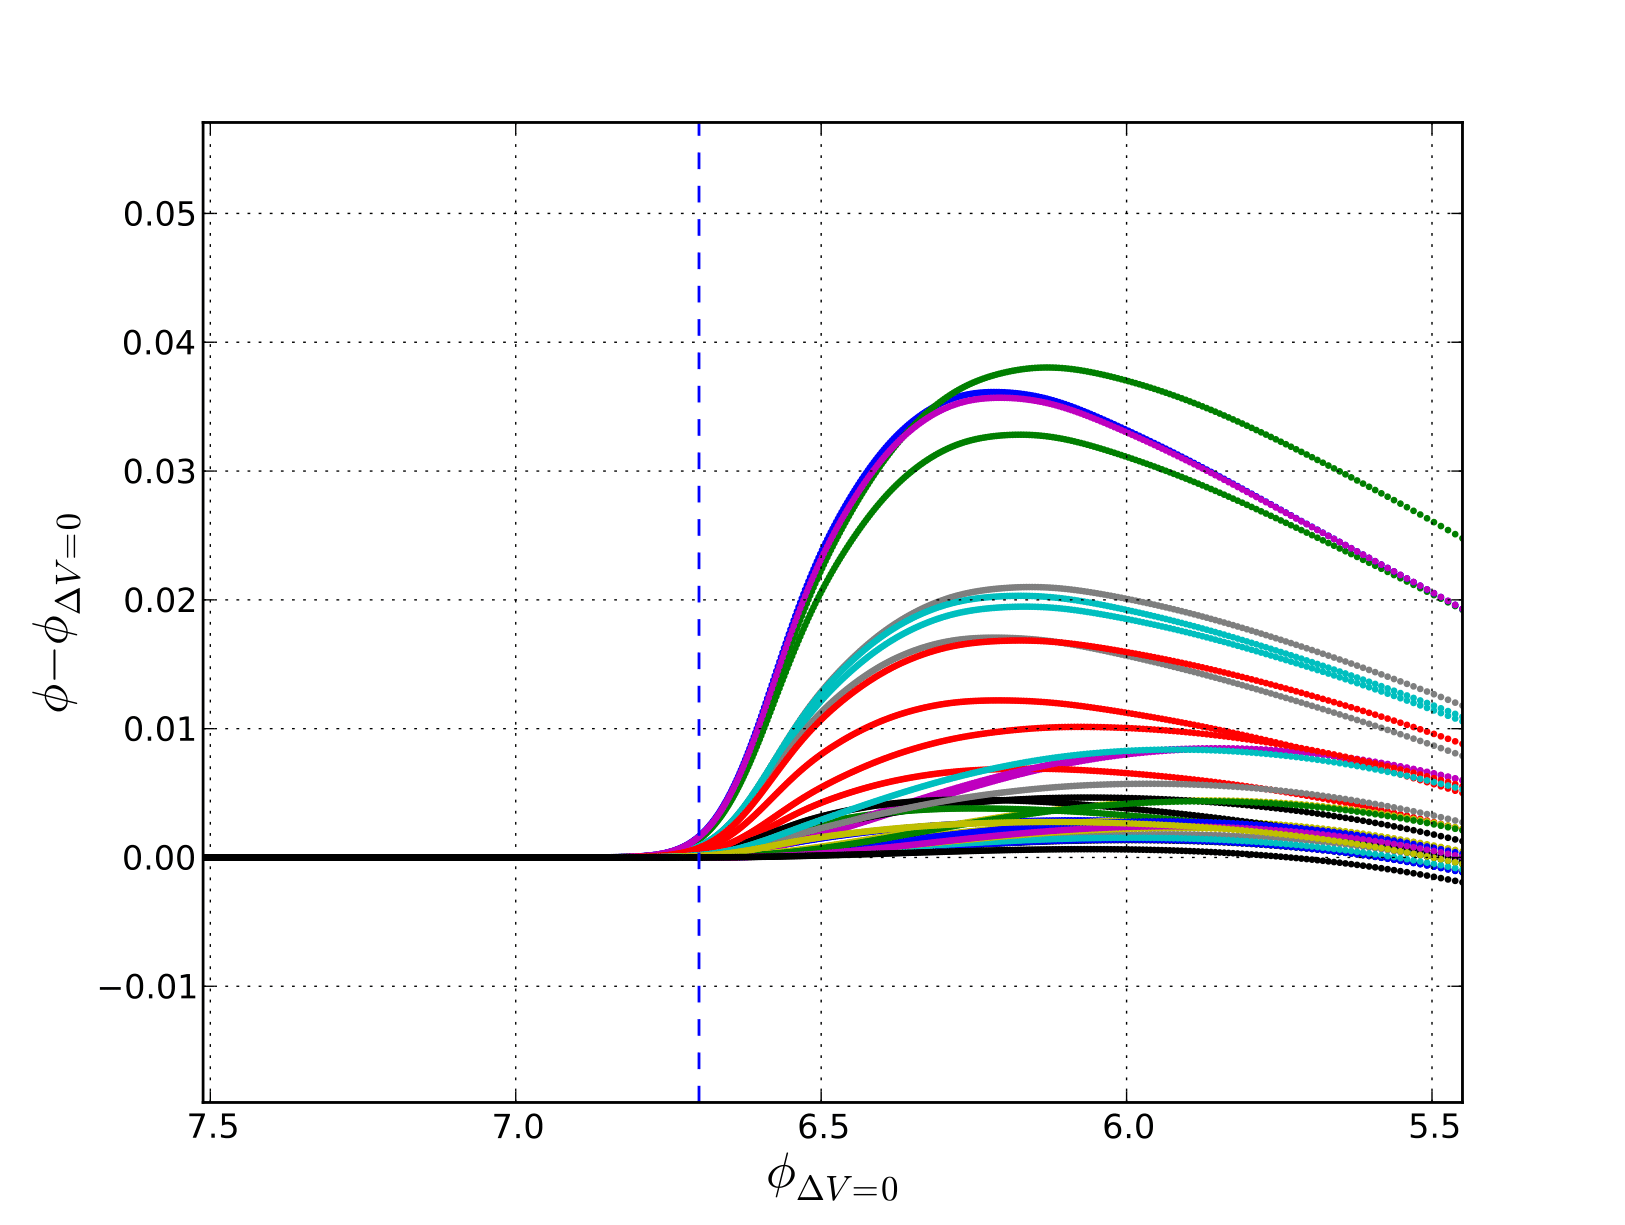
\includegraphics[width=0.75\textwidth]{phi_dif_plot.png}
\caption{The difference between $\phi$ as calculated with and without a $\Delta V$ term in the potential at sampled points on the lattice plotted on the vertical axis, with $\phi$ as calculated without a $\Delta V$ term in the potential along the horizontal axis, the vertical dashed line is located at $\phi=\phi_p$. The separation of trajectories of $\phi$  is due to a secondary effect of the transverse instability causing growth in $\chi$ fluctuations, as $\chi$ fluctuations also cause growth in fluctuations of $V_{,\phi}$ (see (\ref{dv phi})). Trajectories of $\phi$ separate at a delay to those of $\chi$ show in  Figure \ref{chi dv plot}. Fields are in units of $M_{Pl}$.}
% and in contrast with the separation of $\chi$ trajectories}
\label{phi dif plot}
\end{center}
\end{figure}

There is, associated with the transverse instability, a separation of trajectories in the $\phi$ field. As fluctuations of the $\chi$ field grow during the transverse instability $\Delta V_{,\phi}$ becomes more spatially inhomogeneous as well as growing in magnitude. The result is $V_{,\phi}$ becomes less homogeneous and there is a growth of the nonzero Fourier modes of $\phi$. From the slow-roll approximation (\ref{slow roll}) and the form of $V_{,\phi}$, it should be noted that for $\phi<\phi_p$ the larger the fluctuation of $\chi$ at a particular lattice site the more slowly $\phi$ will roll down its potential. This means the effect of $\Delta V$ on the $\phi$ field is to slow its rate of change, but to do so in a way which is inhomogeneous. The separation of $\phi$ trajectories is shown in Figure \ref{phi dif plot}.

%[Talk about production of $\zeta$]

The separation of field values at different comoving positions (lattice sites) shown in Figure \ref{chi dv plot} and Figure \ref{phi dif plot} allows for energy flow to occur between comoving volumes as long as they remain causally connected. The flow of energy between comoving volumes violates the adiabatic assumption used for the derivation of the fluid equation (\ref{fluid eqn}), as previously mentioned in Section \ref{zeta theory}, this leads to the non-conservation of the $\zeta$ parameter. 

Fluctuations of the fields at initial conditions will also lead to non-conservation of $\zeta$. In order to isolate the change in $\zeta$ that is due to the transverse instability two calculations for the evolution of the system are performed from identical initial conditions, one including the $\Delta V$ term in the potential and one setting $\Delta V=0$. Figures \ref{zeta sample plot} and \ref{zeta mean plot} compare the production of $\zeta$ with and without the transverse instability at sampled lattice sites and averaged over the lattice respectively.

\begin{figure}
\begin{center}
%\includegraphics[width=0.75\textwidth]{zeta_sample_plot.pdf}
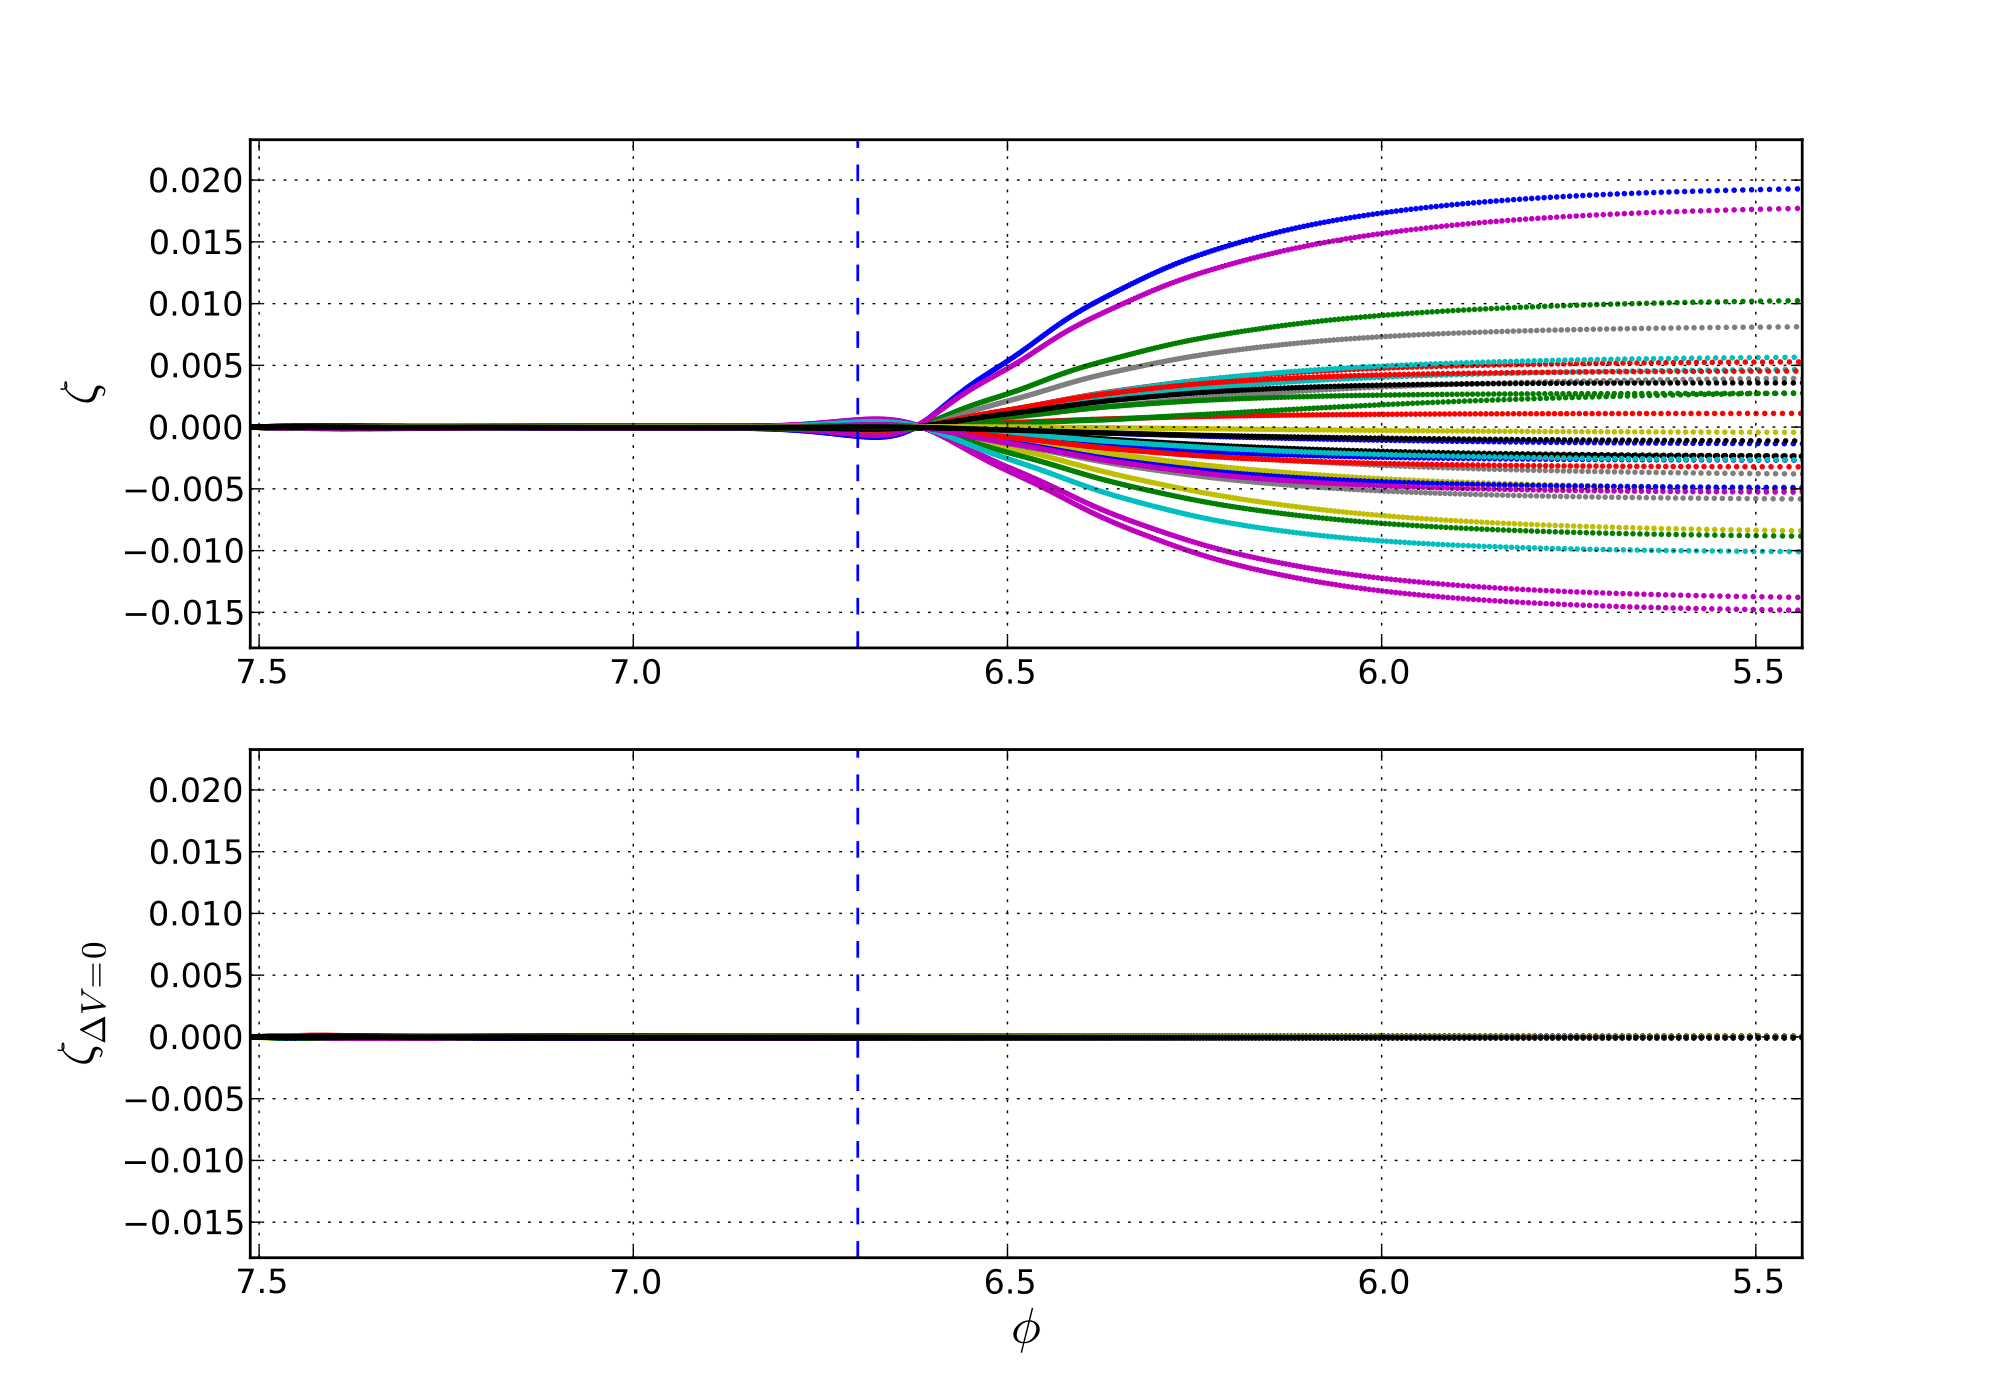
\includegraphics[width=0.75\textwidth]{zeta_sample_plot1.png}
\caption{\emph{Top:} $\zeta$ as calculated at sampled lattice sites with a nonzero $\Delta V$ term included in the potential. \emph{Bottom:} $\zeta$ as calculated at sampled lattice sites with the $\Delta V$ term excluded from the potential.\\
For the top plot the parameters of $\Delta V$ are the same as those used in Figures \ref{chi dv plot} and \ref{phi dif plot}, the vertical dashed line is located at $\phi=\phi_p$. The scales of both the top and bottom plots are the same, demonstrating that a transverse instability during inflation is capable of producing a change in $\zeta$ that is large compared to the change in $\zeta$ caused by the initial fluctuations of the fields, while still allowing inflation to continue in the transverse direction.}
\label{zeta sample plot}
\end{center}
\end{figure}

\begin{figure}
\begin{center}
%\includegraphics[width=0.75\textwidth]{zeta_mean_plot.pdf}
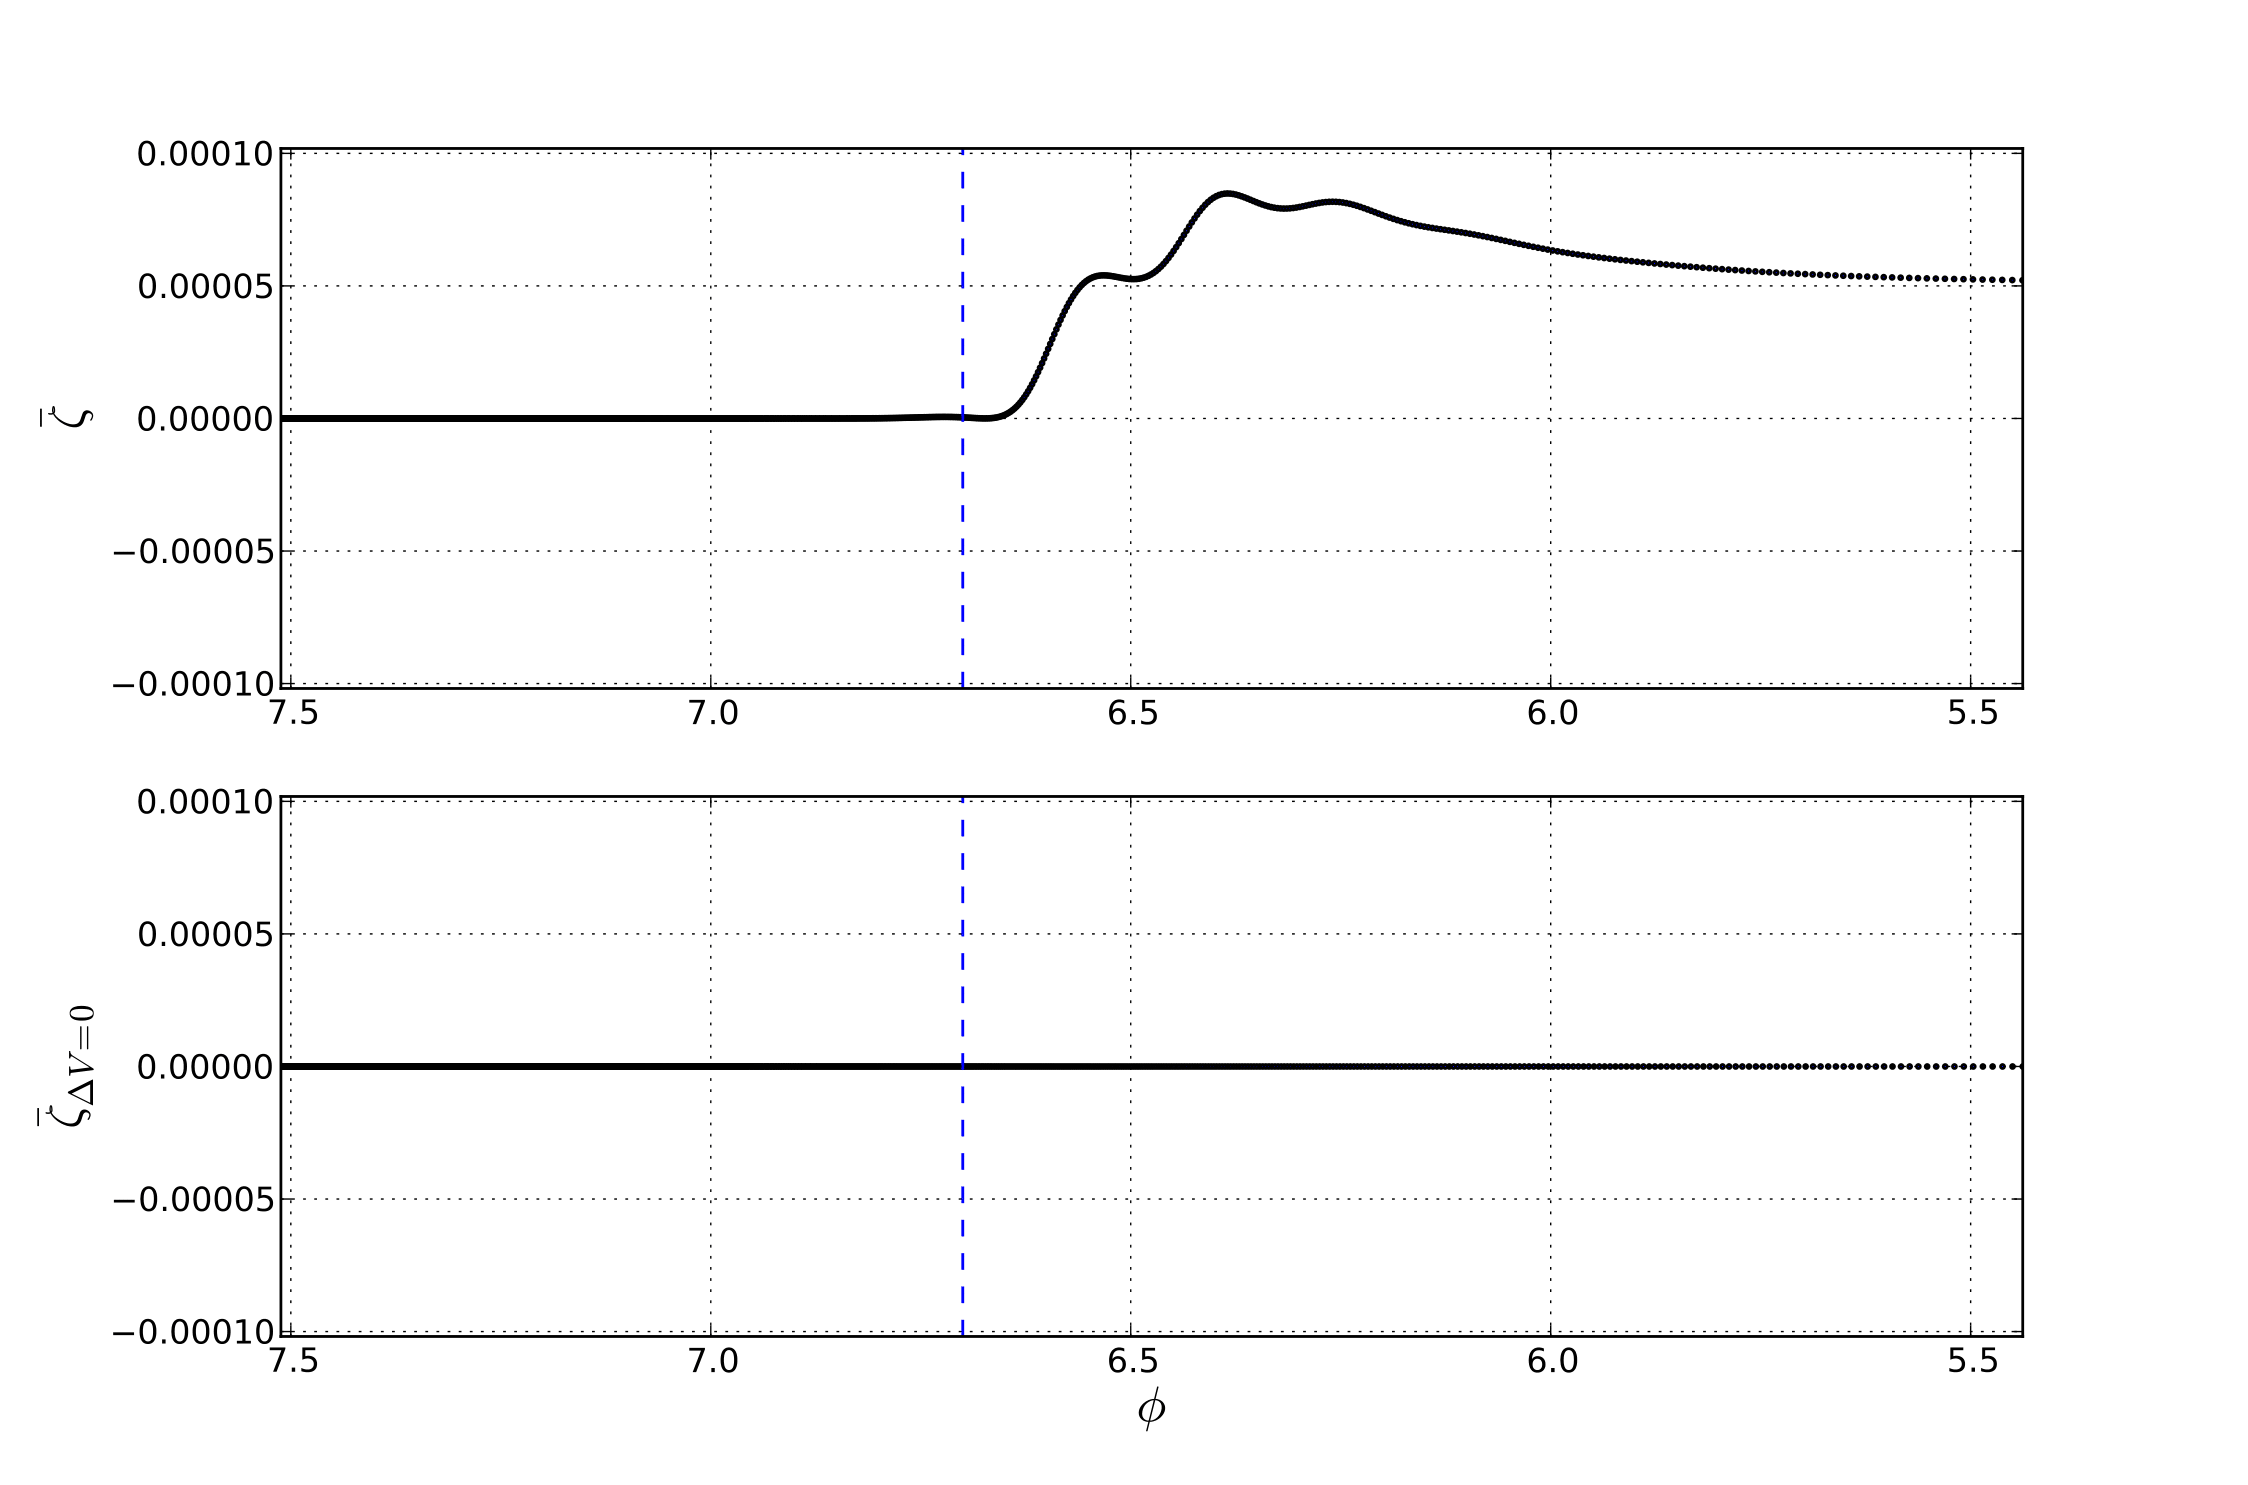
\includegraphics[width=0.75\textwidth]{zeta_mean_plot1.png}
\caption{\emph{Top:} $\zeta$ calculated as an average over the lattice with a nonzero $\Delta V$ term in the potential. \emph{Bottom:} $\zeta$ calculated as an over the lattice with the $\Delta V$ term excluded from the potential.}
\label{zeta mean plot}
\end{center}
\end{figure}

\newpage
\section{Conclusion} \label{conclusion}
We have explored the effects of a temporary transverse instability in a model of two field inflation using a lattice simulation. Using parameters which were selected to allow inflation to continue along the longitudinal direction, the effects of including a $\Delta V$ term in the potential were analyzed for both the transverse and longitudinal field. The change in the $\zeta$ parameter was calculated for the scenario of including a transverse instability, with a baseline established in the absence of such an instability. It was found that the variation in $\zeta$ between lattice sites was greatly enhanced by the inclusion of the $\Delta V$ term to the potential. It remains for future work to determine the post-inflation effects associated with the large production of $\zeta$ varying across the lattice.

%\printbibliography
\bibliography{reportref1}
\bibliographystyle{ieeetr}
\end{document}